\documentclass[12pt]{report}
\usepackage{datetime2}
\renewcommand{\baselinestretch}{1.2} 
\usepackage[breaklinks]{hyperref}
\hypersetup{
    colorlinks,%
    citecolor=black,%
    filecolor=black,%
    linkcolor=black,%
    urlcolor=cyan
}
\author{Siddhant}
\usepackage{listings}
\usepackage{mathpazo}
\usepackage{amsmath}
\usepackage{amssymb}
\usepackage{amsfonts}
\usepackage[utf8]{inputenc}
\usepackage[title,titletoc,toc,page]{appendix}
\usepackage{listings}
\usepackage{graphicx, enumerate,bigints}
\usepackage{amsmath,mathtools}
\usepackage{subfig,morefloats}
\usepackage{epstopdf}
\usepackage{geometry}
\geometry{verbose,tmargin=3cm,bmargin=3cm,lmargin=2.8cm,rmargin=2.8cm}
\setcounter{secnumdepth}{3}
\setcounter{tocdepth}{3}
\usepackage{graphicx,enumerate}
\usepackage{amsmath}
\usepackage{array}
\usepackage{tabularx}
\usepackage{gensymb}
\usepackage{nicefrac}
\usepackage{color}
\usepackage{algorithm}
\usepackage{algpseudocode}
\usepackage{comment}
%\usepackage[toc,page]{appendix}
\makeatletter
\providecommand{\tabularnewline}{\\}
\makeatother
 \usepackage[normalem]{ulem}
 \useunder{\uline}{\ul}{}
  \usepackage{multirow}
% \usepackage[normalem]{ulem}
% \useunder{\uline}{\ul}{}

\usepackage{subfig,morefloats}
\usepackage{booktabs}
\usepackage{fancyhdr}
\usepackage{float}
\usepackage{lastpage}
\usepackage{textcomp}
\definecolor{codegreen}{rgb}{0,0.6,0}
\definecolor{codegray}{rgb}{0.5,0.5,0.5}
\definecolor{codepurple}{rgb}{0.58,0,0.82}
\definecolor{backcolour}{rgb}{0.95,0.95,0.92}

\lstdefinestyle{mystyle}{
    backgroundcolor=\color{backcolour},   
    commentstyle=\color{codegreen},
    keywordstyle=\color{magenta},
    numberstyle=\tiny\color{codegray},
    stringstyle=\color{codepurple},
    basicstyle=\ttfamily\footnotesize,
    breakatwhitespace=false,         
    breaklines=true,                 
    captionpos=b,                    
    keepspaces=true,                 
    numbers=left,                    
    numbersep=5pt,                  
    showspaces=false,                
    showstringspaces=false,
    showtabs=false,                  
    tabsize=2
}

\lstset{style=mystyle}
%\pagestyle{fancyplain}
\fancyhf{}
\newcolumntype{P}[1]{>{\centering\arraybackslash}p{#1}}

\begin{document}
\renewcommand{\arraystretch}{1.5}
\begin{center}
%\vspace*{30pt}
\Large
\textbf{Towards an SoC Architecture for Software-Defined Networking (SDN)}\\
\bigskip
\bigskip
\bigskip
\large
%MTP Stage 1 Report
%\textbf{Master's Thesis Stage - I}\\
%\bigskip
\normalsize
\vspace*{0.5cm}
Dissertation submitted in the fulfillment of  \\
\vspace*{.8cm} \textbf{Master of Technology (M.Tech)}\\
%\vspace*{0.5cm}
by\\
\vspace*{0.5cm}
\textbf{\large Siddhant Singh Tomar} \\
\textbf{Roll No. 213079010}\\


\vspace*{0.5cm}

under the supervision of\\
\textbf{Prof. Madhav P. Desai}\\
\vspace*{1cm}


\vspace*{0.5cm}
\begin{figure}[h!]
 \centering
 
\includegraphics[width=4cm]{../figures/iitb_logo.jpg}
 % emblem.PNG: 124x134 pixel, 72dpi, 4.37x4.73 cm, bb=0 0 124 134
\end{figure}
% \bigskip
\bigskip
%\large
\textbf{Department of Electrical Engineering}\\
\bigskip
\textbf{INDIAN INSTITUTE OF TECHNOLOGY BOMBAY}\\
\textbf{Powai, Mumbai - 400076}\\
\textbf{October 2023}\\
\end{center}
\thispagestyle{empty}

%%%%%%%%%%%%%%%%%%%%%%%%%%%%%%%%%%%%%%%%%%%%%%%%%%%%%%%%%%%%%%%%%%%%%%%%%

\newpage
\pagenumbering{roman}


%%%%%%%%%%%%%%%%%%%%%%%%%%%%%%%%%%%%%%%%%%%%%%%%%%%%%%%%%%%%%%%%%%%%%%%%%
\chapter*{}
\begin{center}
{\Large \textbf{Dissertation Approval}}

\bigskip
\bigskip
\bigskip
This dissertation entitled\\
\bigskip
\textbf{Towards an SoC Architecture for Software-Defined Networking (SDN)}\\
\bigskip

by\\
\bigskip

Mr. Siddhant Singh Tomar\\
Roll No. 213079010\\
\bigskip
is   approved for the degree of\\
\textbf{Master of Technology in Electrical Engineering}\\

\end{center}
 \vspace{10mm}
\begingroup
\setlength{\tabcolsep}{30pt}
\begin{center}
    \begin{tabular}{c c}
        ..................................................... & .....................................................\\
        Prof. Madhav P. Desai & Prof. Virendra Singh\\
        (Supervisor)     & (Examiner)\\
        \\\\
        ..................................................... & .....................................................\\
        Prof. Virendra Singh   & Prof. Sachin B. Patkar\\
        (Chairman) & (Examiner)\\
    \end{tabular}
\end{center}
\endgroup
\bigskip
{Date: \today}\\
{Place: IIT Bombay}


% ------------------------------------------------------------------------------
\newpage








%%%%%%%%%%%%%%%%%%%%%%%%%%%%%%%%%%%%%%%%%%%%%%%%%%%%%%%%%%%%%%%%%%%%%%%%%
\chapter*{}
\begin{center}
{\Large \textbf{Declaration}}
\end{center}
\bigskip
\bigskip
\bigskip
I declare that this written submission represents my ideas in my own words and where
others' ideas or words have been included, I have adequately cited and referenced the sources.  
I also declare that I have adhered to all principles of academic honesty and integrity
and   have   not   misrepresented   or   fabricated   or   falsified   any   idea/data/fact/source   in   my
submission.  I understand that any violation of the above will be cause for disciplinary action
by the Institute and can also evoke  penal action from the sources which have thus not been
properly cited or from whom proper permission has not been taken when needed.\\
\bigskip
\bigskip
\bigskip
\begin{flushleft}
..................................\\
{Mr. Siddhant Singh Tomar\\
Roll No. 213079010}
\end{flushleft}

\begin{flushleft}
{Date : \today}
\end{flushleft}

% ------------------------------------------------------------------------------
\newpage

\chapter*{}
\begin{center}
{\Large \textbf{Acknowledgment}}
\end{center}
I want to express my heartfelt gratitude towards \textbf{Prof. Madhav P. Desai} for allowing me to work on this project and providing her valuable guidance throughout. His suggestions have helped me in gaining a better understanding of this research topic. Lastly, I am perpetually thankful to my family and friends for their unwavering encouragement and support.
% --------------------------------------------------------------------------------

\newpage

\chapter*{}
\begin{center}
{\Large \textbf{Abstract}}
\end{center}

In this thesis, we describe the design and implementation of a System on Chip (SoC) platform for Software-Defined Networking (SDN). The SoC integrates a 32-bit AJIT processor with a custom network interface controller (NIC) and high-capacity main memory (DRAM). The entire SoC was implemented and validated on a Xilinx KC705 FPGA. To characterize the performance of the SoC, we used two applications: Ping and Network Content Cache, utilizing the open-source TCP/IP stack called LwIP. 

Our findings indicate that the performance of these applications is influenced by the architecture of the memory subsystem. To enhance the SoC's performance, we explored two memory subsystem architectures between the NIC and the processor. The first architecture employs a fast local packet memory shared by both the processor and the NIC. The second architecture uses L2 cache in the processor and NIC's access path to the main memory. Both architectures resulted in performance improvements, with the first architecture performing better for the applications considered. Thus, the first architecture can serve as a foundational design for SoCs aimed at high-performance networking, with potential for further optimizations.\\
\par
 
%%%%%%%%%%%%%%%%%%%%%%%%%%%%%%%%%%%%%%%%%%%%list of figures

\tableofcontents
\newpage
%\pagenumbering{arabic}
\addcontentsline{toc}{chapter}{\listfigurename}
\listoffigures
\newpage
\addcontentsline{toc}{chapter}{\listtablename}
\listoftables
%\lipsum[1-20]
%\newpage                     A three-line code for empty page insertion
%\thispagestyle{empty}
%\mbox{}



\newpage

\clearpage




\pagenumbering{arabic}
\chapter{Introduction} \label{1}
%\label{ch:intro}
\rule[10pt]{\linewidth}{3pt}
 
\section{Introduction}



The advent of Software-Defined Networking (SDN) has revolutionized network design, management, and optimization. By decoupling the control plane from the data plane, SDN allows for more flexible and dynamic network management. As SDN continues to evolve, the demand for efficient and high-performance System-on-Chip (SoC) platforms tailored for SDN applications has surged. \\ \\
In this thesis, we have focussed on the design and implementation of such an SoC platform, which can provide computing, networking, and storage capabilities for SDN applications. The SoC platform includes a 32-bit AJIT processor integrated with a custom network interface controller (NIC) and a large-capacity main memory (DRAM). This entire SoC setup was implemented and validated on a Xilinx KC-705 FPGA. To assess the performance of the SoC, we employed two applications—Standard Ping and Network Content Caching. We verified the two applications in a bare-metal environment, utilizing the lwIP (lightweight IP) open-source TCP/IP stack, which was ported for the AJIT processor and custom NIC. 
lwIP (lightweight IP) is a widely used open-source TCP/IP stack designed for embedded systems. \\ \\
\newpage
We have studied the impact of the memory subsystem architecture on the performance of these two applications. To enhance the overall data plane performance, we investigated two modifications to the memory subsystem architecture.
The first architecture employs a fast local packet memory shared by both the processor and the NIC. The second architecture uses L2 cache in the processor and NIC's access path to the main memory. \\ 
Both architectures demonstrated performance improvements. Specifically, the first architecture achieved a 34.5\% speedup, while the second architecture realized a 18.3\% speedup in the considered applications compared to our baseline architecture. Therefore, the first architecture is recommended for designing the memory subsystem to ensure sufficient fast buffering for packets in the data plane. \\ 
Further optimization opportunities can be explored by enhancing the architecture to offload additional computational tasks to the NIC. This approach could streamline processing within the SoC, leveraging the NIC's capabilities to handle specific tasks more efficiently.

\section{Objectives}

This research aimed to develop an SoC architecture capable of integrating computing, networking, and storage functionalities for SDN applications. This SoC includes a single-core 32-bit AJIT processor, along with a custom-designed NIC and DRAM subsystem for storage.
The architecture of this SoC serves as a foundational framework for constructing more advanced SoCs featuring multiple processor cores and NICs for high-performance networking and further research. \\

\section{Organization of the thesis}
In Chapter 2 of this thesis, the detailed organization and performance characterization of the baseline SoC architecture, specifically the single board computer (SBC), are presented. In Chapter 3, we discuss the optimizations made to the baseline architecture, with a focus on the memory subsystem, and provide their performance characterization. In Chapter 4, a comparative analysis of the three architectures is conducted, along with a discussion on future work for further optimization. The Appendix contains the detailed design of the NIC and the network caching application.












%\section{Objective}
%%%%%%%%%%%%%%%%%%%%%%%%%%%%%%%%%%%%%%%%%%%%%%%%%%%%%%%%%%%%%%%%%%%%%%%%%%%%%%%%%%%%%%%%
\newpage
\chapter{Baseline Architecture of the SoC}
\rule[10pt]{\linewidth}{3pt}
\section{Introduction}

This chapter includes a detailed description of the baseline architecture of the SoC, which is essentially a single-board computer (SBC), incorporating a 32-bit AJIT processor integrated with a custom-designed network interface controller (NIC) and a memory subsystem (DRAM), together with some peripherals.
This chapter also gives a brief description of the custom NIC, designed by Harshad Ugale at IITB, which was modified and optimized as part of this project. The integration and working of the NIC with the rest of the SoC is thoroughly discussed. The SoC described in this chapter, will serve as the template for further system/architecture exploration. The architecture presented here will serve as the baseline for comparison with other memory subsystem architectures.


\begin{figure}[h]
			\centering
			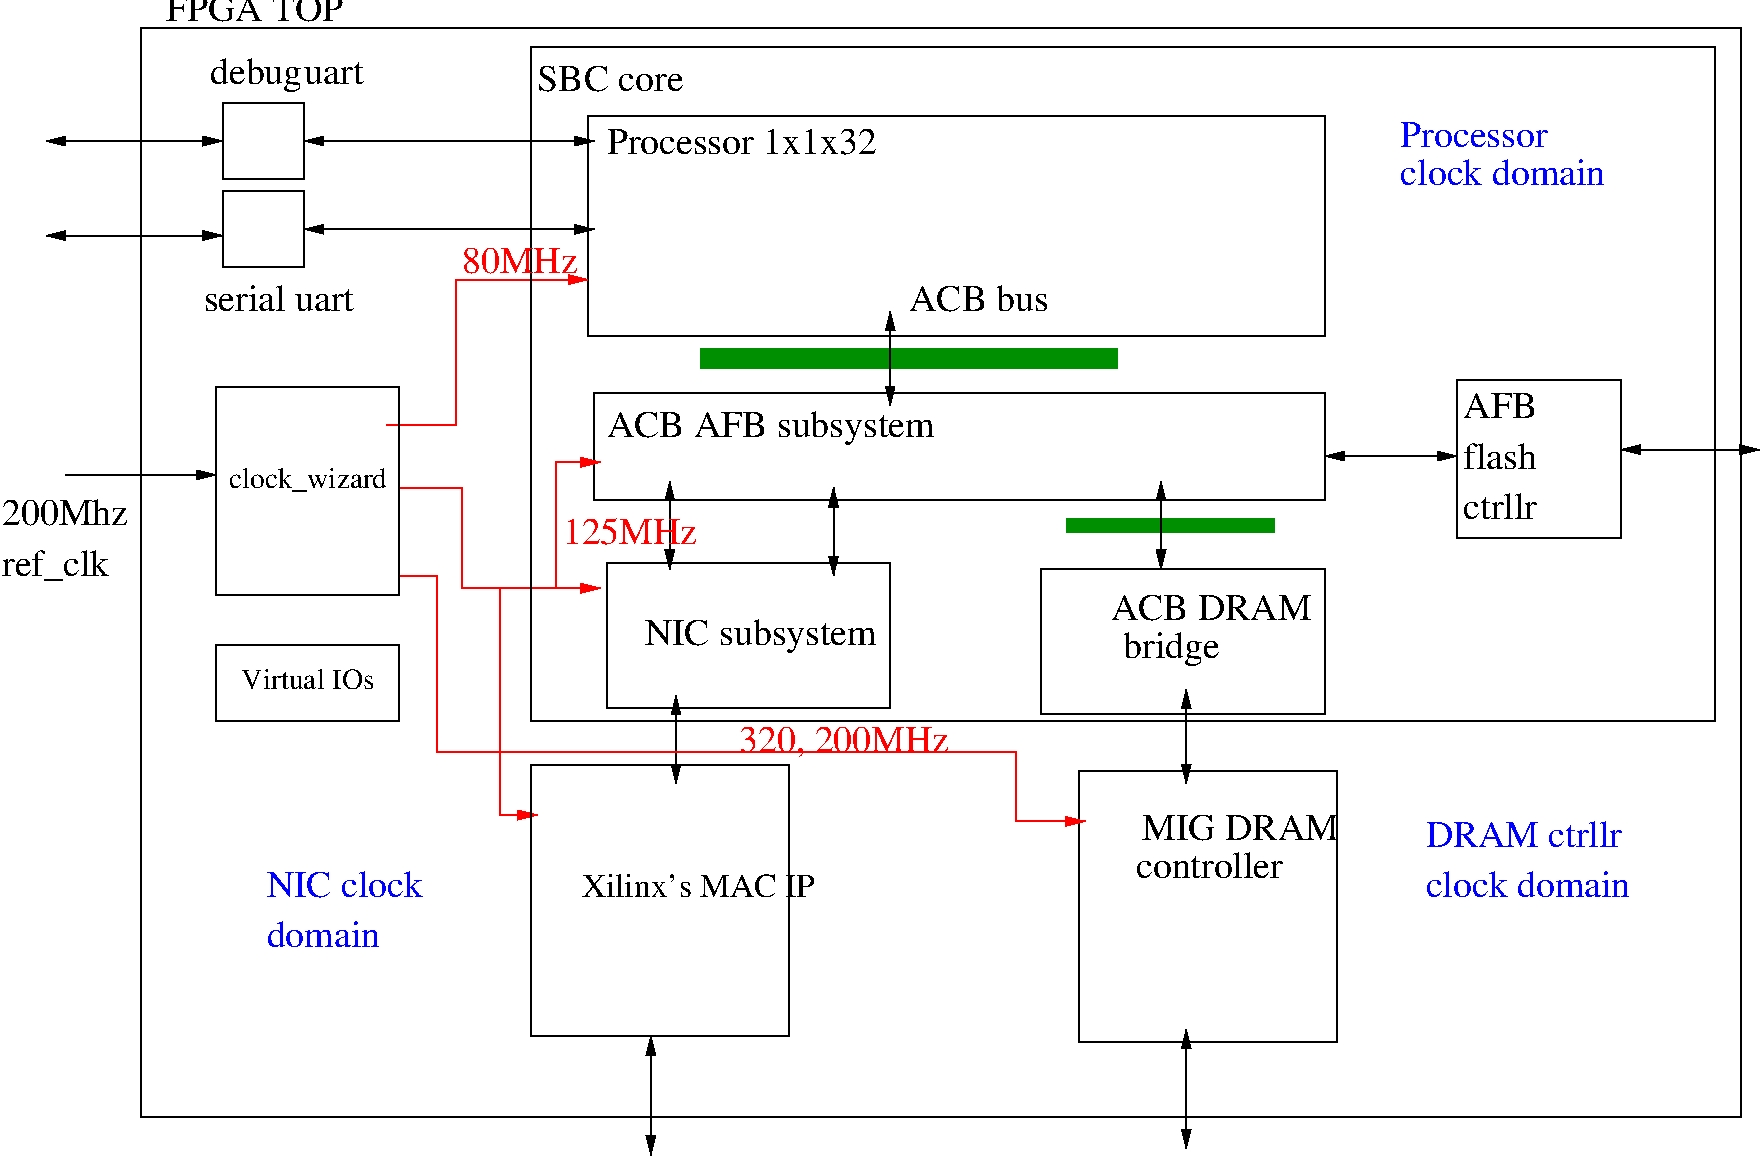
\includegraphics[width=14cm]{../figures/FINAL_SBC.jpg}
			\caption{Architecture of single board computer with AJIT 1x1x32}
			\label{fig:NIC-Proc-top1}
		\end{figure}
\section{The Single board computer (SBC)}
The architecture of a single-board computer (SBC) is organized into a "SBC core" and a "SBC periphery" as shown in Figure 2.1. The "core" comprises a single-threaded 32-bit AJIT processor, a custom-designed NIC, an ACB, and an AFB bus complex. The "periphery" includes the Xilinx tri-mode Ethernet MAC IP, which interfaces with both the NIC subsystem in the core and the PHY on the FPGA, and the Xilinx MIG DRAM controller IP, which connects to the ACB DRAM bridge in the core and manages the DRAM memory on the FPGA..
\section{SBC Core}

The main subsystems of the "core" in SBC are as follows:
\begin{enumerate}
    \item AJIT (1x1x32) processor subsystem. 
    \item Custom Network Interface Controller (NIC) subsystem.
    \item Bus complex consisting of 32-bit AFB and 64-bit ACB buses.
\end{enumerate}

\subsection{Processor 1x1x32}
\begin{figure}[h]
			\centering
			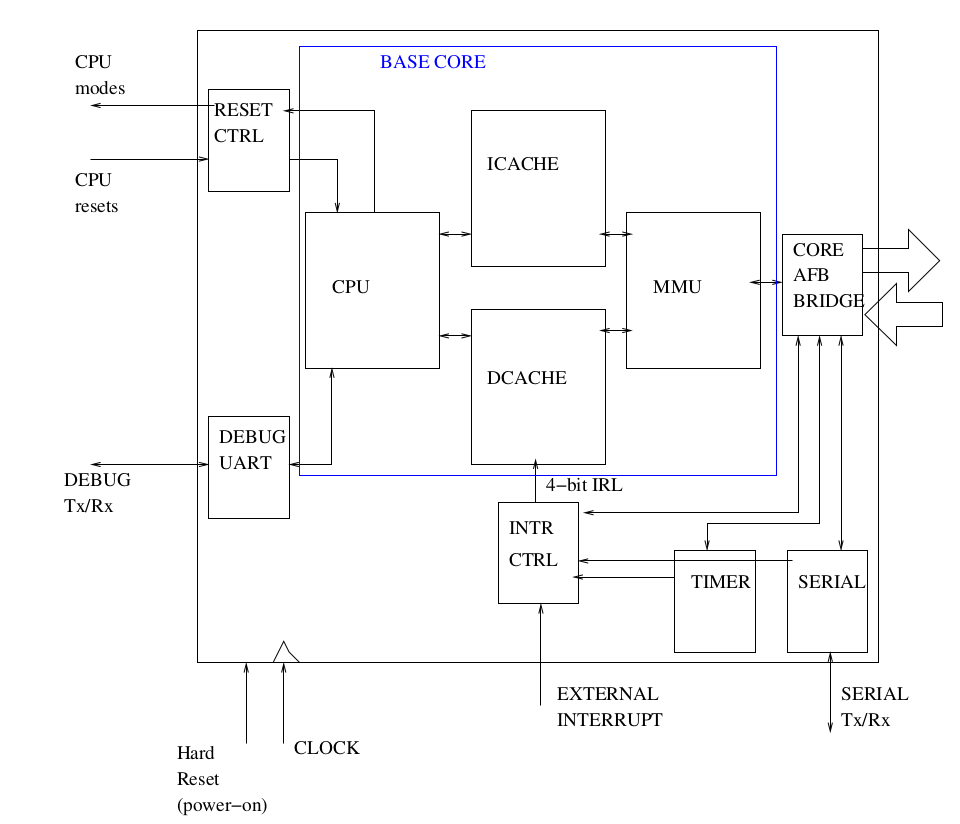
\includegraphics[width=12cm]{../figures/proc.png}
			\caption{The Generic 32-bit AJIT processor core}
			
		\end{figure}
\begin{enumerate}
    \item AJIT processor central processing unit (CPU): implements the SPARC-V8
ISA (Draft IEEE standard 1754-1996).
\item  Instruction Cache (ICACHE): A 32-kB (64-byte line size), direct mapped,
virtually indexed, and virtually tagged instruction cache.
\item Data Cache (DCACHE): A 32-kB (64-byte line size), direct mapped, vir-
actually indexed and virtually tagged data cache with write-through allocate
policy.
\item  Memory management unit (MMU): implements all required aspects of the
SPARC reference MMU. A 64-bit AJIT Core Fifo Bus interface is provided.

\end{enumerate}

\subsection{NIC subsystem}
The NIC subsystem comprises the custom-designed NIC and NIC-TO-MAC-BRIDGE.
\begin{figure}[h]
			\centering
			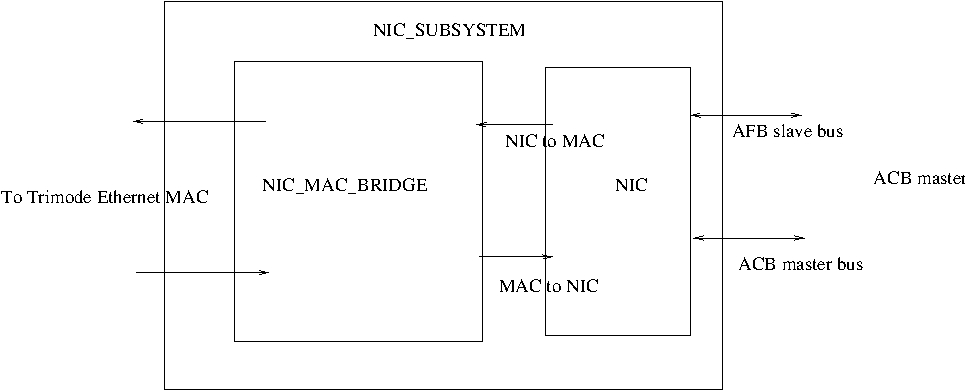
\includegraphics[width=10cm]{../figures/NIC_SUBSYSTEM.jpg}
			\caption{NIC Subsytem}
		\end{figure}

The various interfaces that NIC exposes to rest of the SoC are discussed below:\\
\begin{enumerate}
    \item \textbf{Processor to NIC slave interface}:
The processor will allocate memory regions from the address space for packet buffers and queue data structures that hold pointers to these packet buffers. It also configures the NIC's registers with the physical addresses of the queue data 

\item \textbf{NIC to Memory master interface}:
 The queues are populated with the physical addresses of the packet buffers, allowing the NIC to write directly to the main memory using the ACB (AJIT CORE Bus 64-bit) protocol. 

 \item \textbf{NIC subsystem To MAC interface}:
The NIC subsystem is linked to a tri-mode Ethernet MAC IP to capture Ethernet frames via the NIC-MAC bridge. Tri-mode Ethernet MAC IP connects to ethernet PHY on the FPGA.
\end{enumerate}

  
\subsection{ACB AFB Bus Complex}
The primary interfaces between the AJIT processor and the external
world are:
\begin{enumerate}
    \item AJIT CORE BUS interface (ACB): A 64-bit data, 36-bit address system memory interface.
    \item AJIT FIFO BUS interface (AFB): A 32-bit data, 36-bit peripheral/memory
interface.
\end{enumerate}

Both these bus interfaces involve a request and a response interface. The
bus master sends a request word to the slave, which responds to the request
with a response word. The exchange of data between the master and slave
is regulated using a simple two-wire protocol.

\begin{figure}[h]
			\centering
			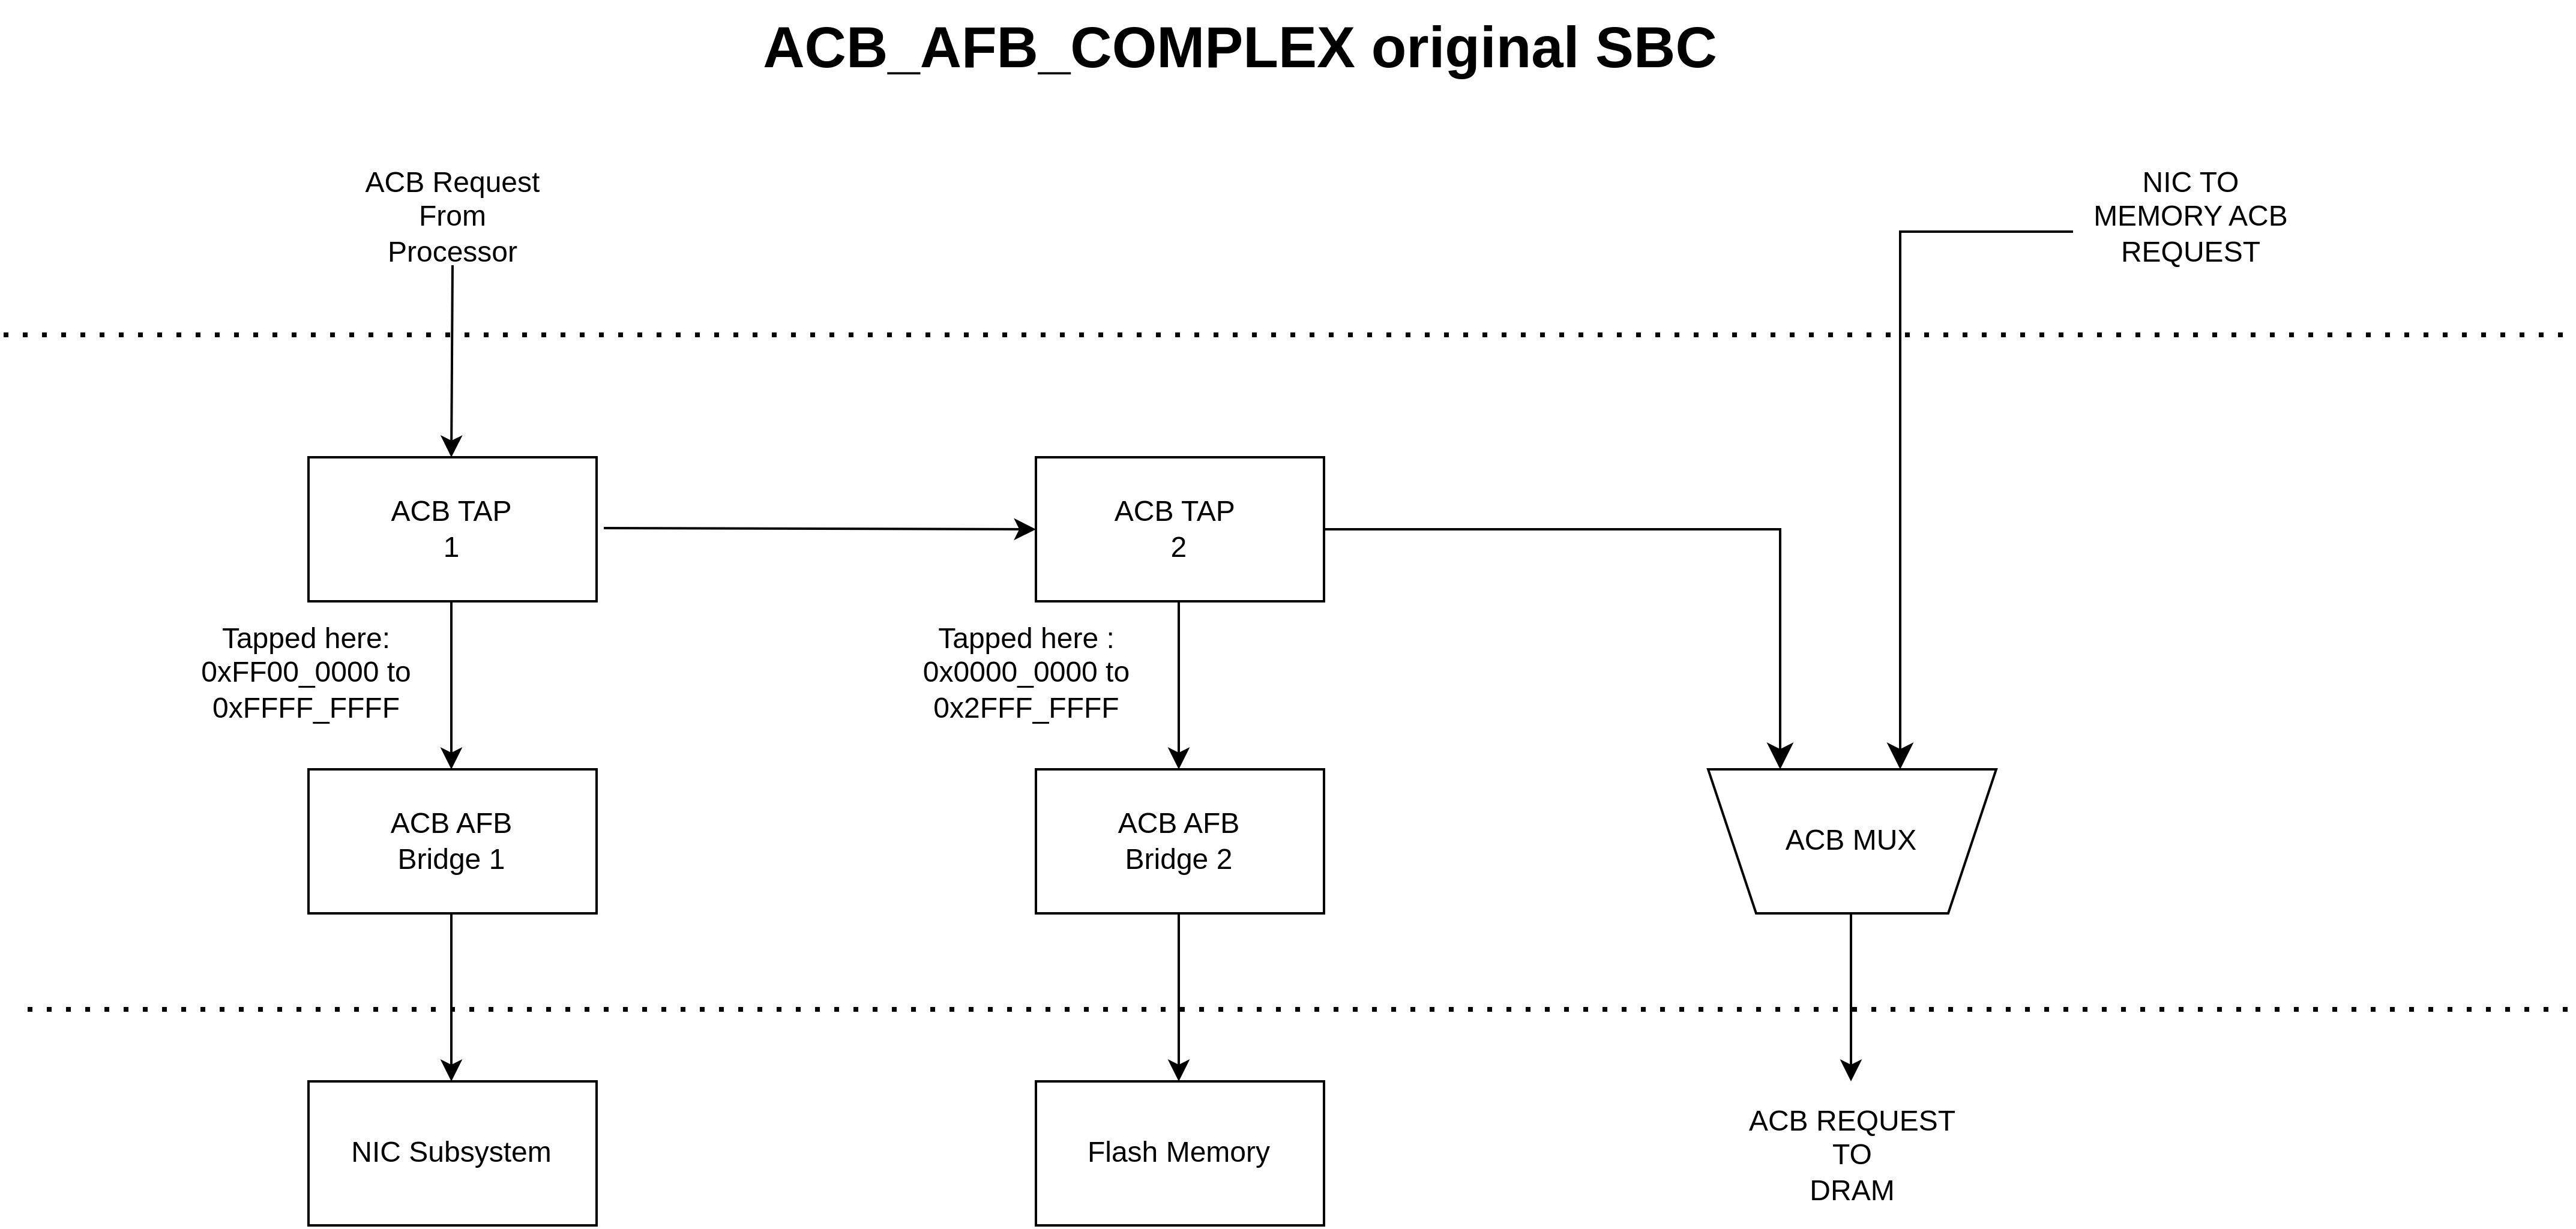
\includegraphics[width=16cm]{../figures/acb_afb_complex.jpg}
			\caption{ACB AFB bus complex.}
			
		\end{figure}

\newpage
\section{SBC periphery}
The peripherals contain the Xilinx IPs used in the SBC:
\begin{enumerate}
    \item Xilinx Tri-mode ethernet MAC IP   
    \item Xilinx MIG DRAM controller IP
\end{enumerate}
\subsection{Xilinx tri-mode ethernet MAC IP}

The block diagram above shows the various elements of the example design and where they physically reside. Here is a basic
description of the significant blocks and their purpose in the design. The Tri-Mode Ethernet Media Access Controller (TEMAC) solution comprises the 10/100/1000 Mb/s and 10/100 Mb/s Intellectual Property (IP) cores along with the optional Ethernet AVB Endpoint which are fully verified designs. A MAC is responsible for the Ethernet framing protocols and error detection of these frames. The MAC is independent of, and can be connected to, any type of physical layer.

\begin{figure}[h]
			\centering
			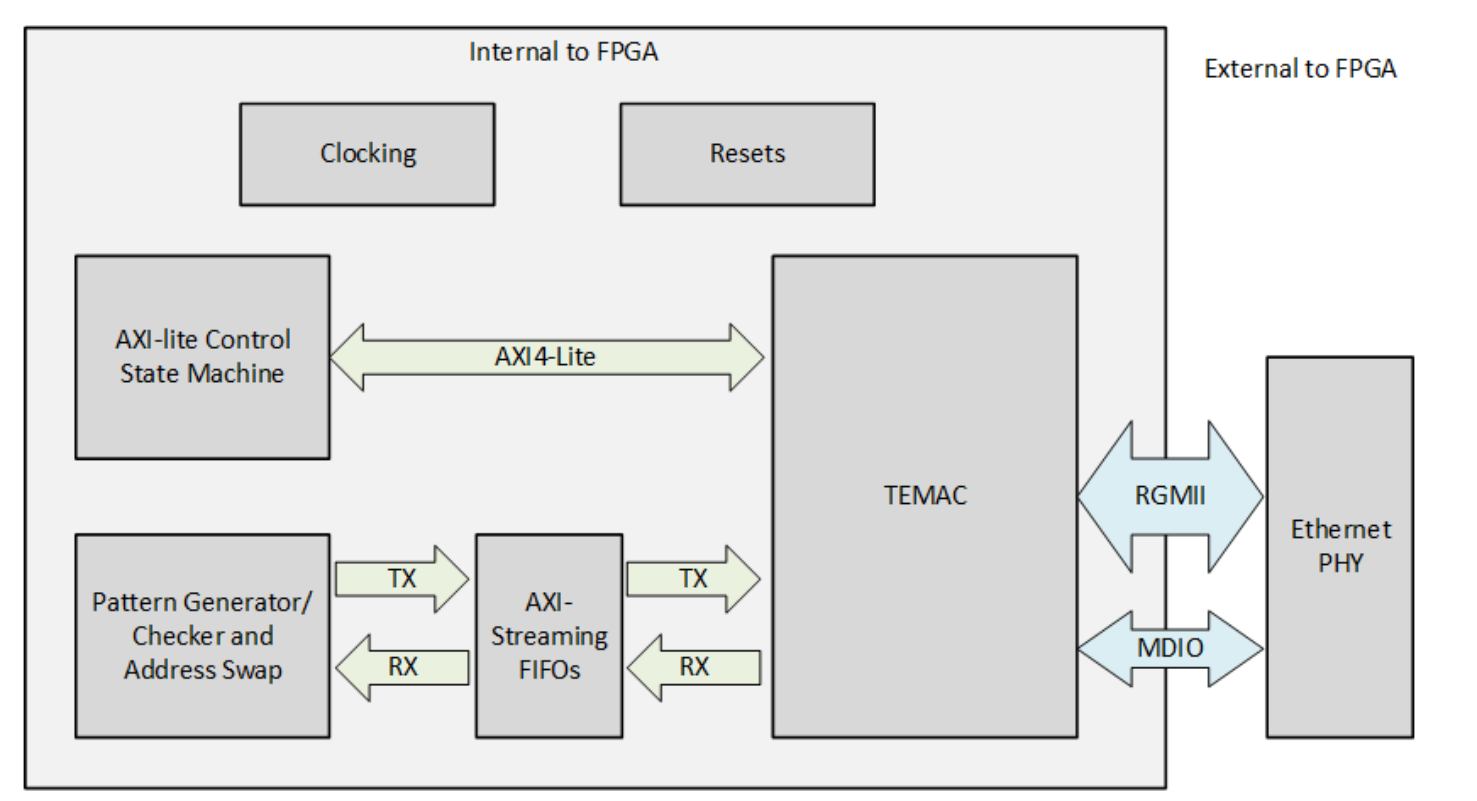
\includegraphics[width=14cm]{../figures/MAC_IP.png}
			\caption{Block diagram of the Trimode MAC IP.}
			
		\end{figure}

\begin{enumerate}

    \item \textbf{TEMAC}: The Tri-Mode Ethernet MAC implements the MAC (media access control) layer of the IP stack, a sublayer of the data link layer.

    \item \textbf{AXI-lite Control State Machine}: The state machine performs basic transactions over the AXI-lite interface of the TEMAC, and brings up the MAC and the external Ethernet PHY to allow basic frame transfer.

    \item \textbf{AXI-Streaming FIFOs}: The FIFOs add buffering between the TEMAC and the packet generator/checker. 
    
\end{enumerate}

\subsection{Xilinx MIG DRAM controller IP}
The MIG 7 Series DDR3/DDR2 LogiCORE IP is provided as a full memory interface design with a physical layer (PHY), a highly efficient memory controller, and user interface blocks. All blocks are provided as HDL source code. Xilinx supports using the PHY-only portion of the MIG 7 Series IP to interface with the custom controller.

\section{Clock Domains in SBC}
The single-board computer (SBC) is designed with two distinct clock domains. The Processor subsystem and DRAM memory subsystem operate at 80MHz, and the NIC subsystem operates at 125MHz. To facilitate the connection between these subsystems, Dual Clock asynchronous FIFOs are employed (depicted as green boxes in Figure 2.1), one for ACB Request and another for ACB Response. The system is organized in a manner that minimizes the quantity of FIFOs needed. Clock signals are distributed throughout the system via clock wizard IPs.


\section{System organization: Working of Processor and NIC in packet processing}
This section provides an overview of the mechanisms in packet reception and transmission, involving a Network Interface Card (NIC) and the processor.
\subsection{Packet Reception}
In packet reception, the processor, through the driver code, interacts with the Network Interface Card (NIC) to manage the flow of incoming network packets. The processor and NIC utilize a system of packet descriptors organized in rings within the main memory (DRAM).
\begin{enumerate}
    \item Packet Descriptor Rings: The processor, specifically the driver code, maintains rings of packet descriptors in DRAM. These descriptors are essentially metadata structures that describe where packet data should be stored.

    \item Initialization with Empty Buffers: The driver populates these descriptor rings with pointers to empty packet buffers. These buffers are areas in memory where incoming packet data will be stored.

    \item NIC Data Writing Process: When a packet arrives, the NIC takes an empty buffer pointer from a structure known as the "receive free queue". The NIC then writes the incoming packet data directly into the buffer in main memory. After filling the buffer, the NIC moves the buffer pointer to the "receive queue".

    \item Processor Polling: The processor continuously polls the receive queue for new packets. Once it finds a filled buffer pointer, it reads the data from the buffer, processes the packet, and then returns the buffer pointer to the free queue, readying it for the next incoming packet.
\end{enumerate}

This process ensures an efficient and continuous flow of data from the network into the system's main memory, allowing the processor to handle packets as they arrive.

\subsection{Packet Transmission}

For packet transmission, the roles of the processor and NIC are somewhat reversed, but the underlying principles of using descriptor rings and queues remain the same.
\begin{enumerate}
    \item Packet Descriptor Rings: As with reception, the processor's driver code maintains rings of packet descriptors in DRAM for outgoing packets.

    \item Initialization with Empty Buffers: The driver also initializes these rings with pointers to empty packet buffers.

    \item Processor Data Writing Process: When the processor has data to send, it takes an empty buffer pointer from the "transmit free queue", writes the data into the buffer in main memory, and then places the buffer pointer into the "transmit queue".

    \item NIC Polling: The NIC continuously polls the transmit queue for buffers containing data ready to be sent. When it finds one, it transmits the packet over the network and then returns the buffer pointer to the free queue.
\end{enumerate}


This mechanism ensures that data is efficiently transferred from the system's memory to the network, leveraging the NIC's capabilities to handle the actual transmission.

\section{Performance Characterization of Baseline SoC}
The SoC was implemented and validated on KC-705 FPGA.
The performance of the SoC was characterized using two applications, namely the standard Ping application and the Network content cache application. Both the applications were executed in a bare-metal environment using an open-source TCP/IP stack, lwIP(lightweight IP), which was ported for the AJIT processor and custom-designed NIC. 

\subsection{Average round trip time (RTT)}
To measure the average RTT, ICMP request packets were generated using the standard ping command from a Linux terminal on a host machine and sent to the SoC on the FPGA. The processor core was running at 80MHz, the NIC subsystem operated at 125MHz with a 1Gbps Ethernet link, and the lwIP TCP/IP stack generated ICMP response packets.

\begin{table*}[h!]
\caption{Avg RTT time and Data rate achieved for different  packet sizes}
\begin{center}
\begin{tabular}{|c|c|}

\hline
\textbf{Packet size(bytes} & \textbf{Average RTT (us)}  \\
\hline
64 & 290    \\
\hline
128 & 354   \\
\hline
256 & 388   \\
\hline
512 & 429   \\
\hline
1024 & 449   \\
\hline
\end{tabular}
\label{table_dataRate}
\end{center}
\end{table*}



\newpage
\subsection{Network Content Caching application}

In this application, the SoC setup is deployed on the FPGA, where both the lwIP server and client are running. Two hosts, A and B, are operating on the host side (PC or laptop). Host A pre-populates the cache (DRAM) with frequently needed data via a TCP connection. When Host B requests data from Host A, Host A sends a "forward" command to the lwIP server on the FPGA, including Host B's IP address and port number. The lwIP server then forwards the data to Host B using a UDP connection. The data transmission speeds for populating the "cache" on the FPGA by Host A and forwarding data from the "cache" on the FPGA to Host B are reported below.
\begin{enumerate}
    \item Host A(on PC) to Controller (On FPGA): 23.7 Mbps
    \item Controller (On FPGA) to Host B (on PC) : 13.43 Mbps
\end{enumerate}
(\textbf{Application is described in more detail in appendix B})


\section{Epilogue}
To improve the performance of the aforementioned applications, we have explored enhancements to the memory subsystem architecture. \newline \textbf{Two optimizations will be detailed in the following chapter}
%%%%%%%%%%%%%%%%%%%%%%%%%%%%%%%%%%%%%%%%%%%%%%%%%
\newpage

\chapter{Optimization of the Baseline Architecture}
\section{Introduction}
\rule[10pt]{\linewidth}{3pt}

In our efforts to optimize the baseline architecture, we have focused on enhancing the memory subsystem architecture. This component lies along the data plane path of packet processing and represents a crucial pathway where significant performance improvements can be achieved. We
investigated two modifications to the memory subsystem architecture first architecture employs a fast local packet memory shared by both the processor and the NIC. The second architecture uses an L2 cache in the processor and NIC's access path to the main memory. Both the optimization and their impact are detailed in this chapter

\section{Optimization A: Sharing a fast local packet memory between the NIC and the processor}

The proposed architecture suggests a departure from the conventional approach of storing descriptor ring structures and packet buffers in the slower main memory (DRAM). Instead, these critical components are housed within a fast local memory that is shared between the processor and the Network Interface Card (NIC). Importantly, this shared memory region is designated as non-cacheable to ensure consistent states.

By leveraging a fast local memory, the architecture aims to significantly reduce access latency for both the processor and the NIC. This memory is optimized for speed, making it ideal for storing time-sensitive data structures like descriptor rings and packet buffers.
Placing the descriptor rings and packet buffers in a shared memory space facilitates efficient communication and data transfer between the processor and the NIC. This shared resource allows both entities to access and modify data quickly without the overhead typically associated with accessing DRAM. By reducing memory access latency and optimizing data-sharing mechanisms, the proposed architecture aims to enhance the system's overall performance and throughput. The architecture is shown below.

	\begin{figure}[h]
			\centering
			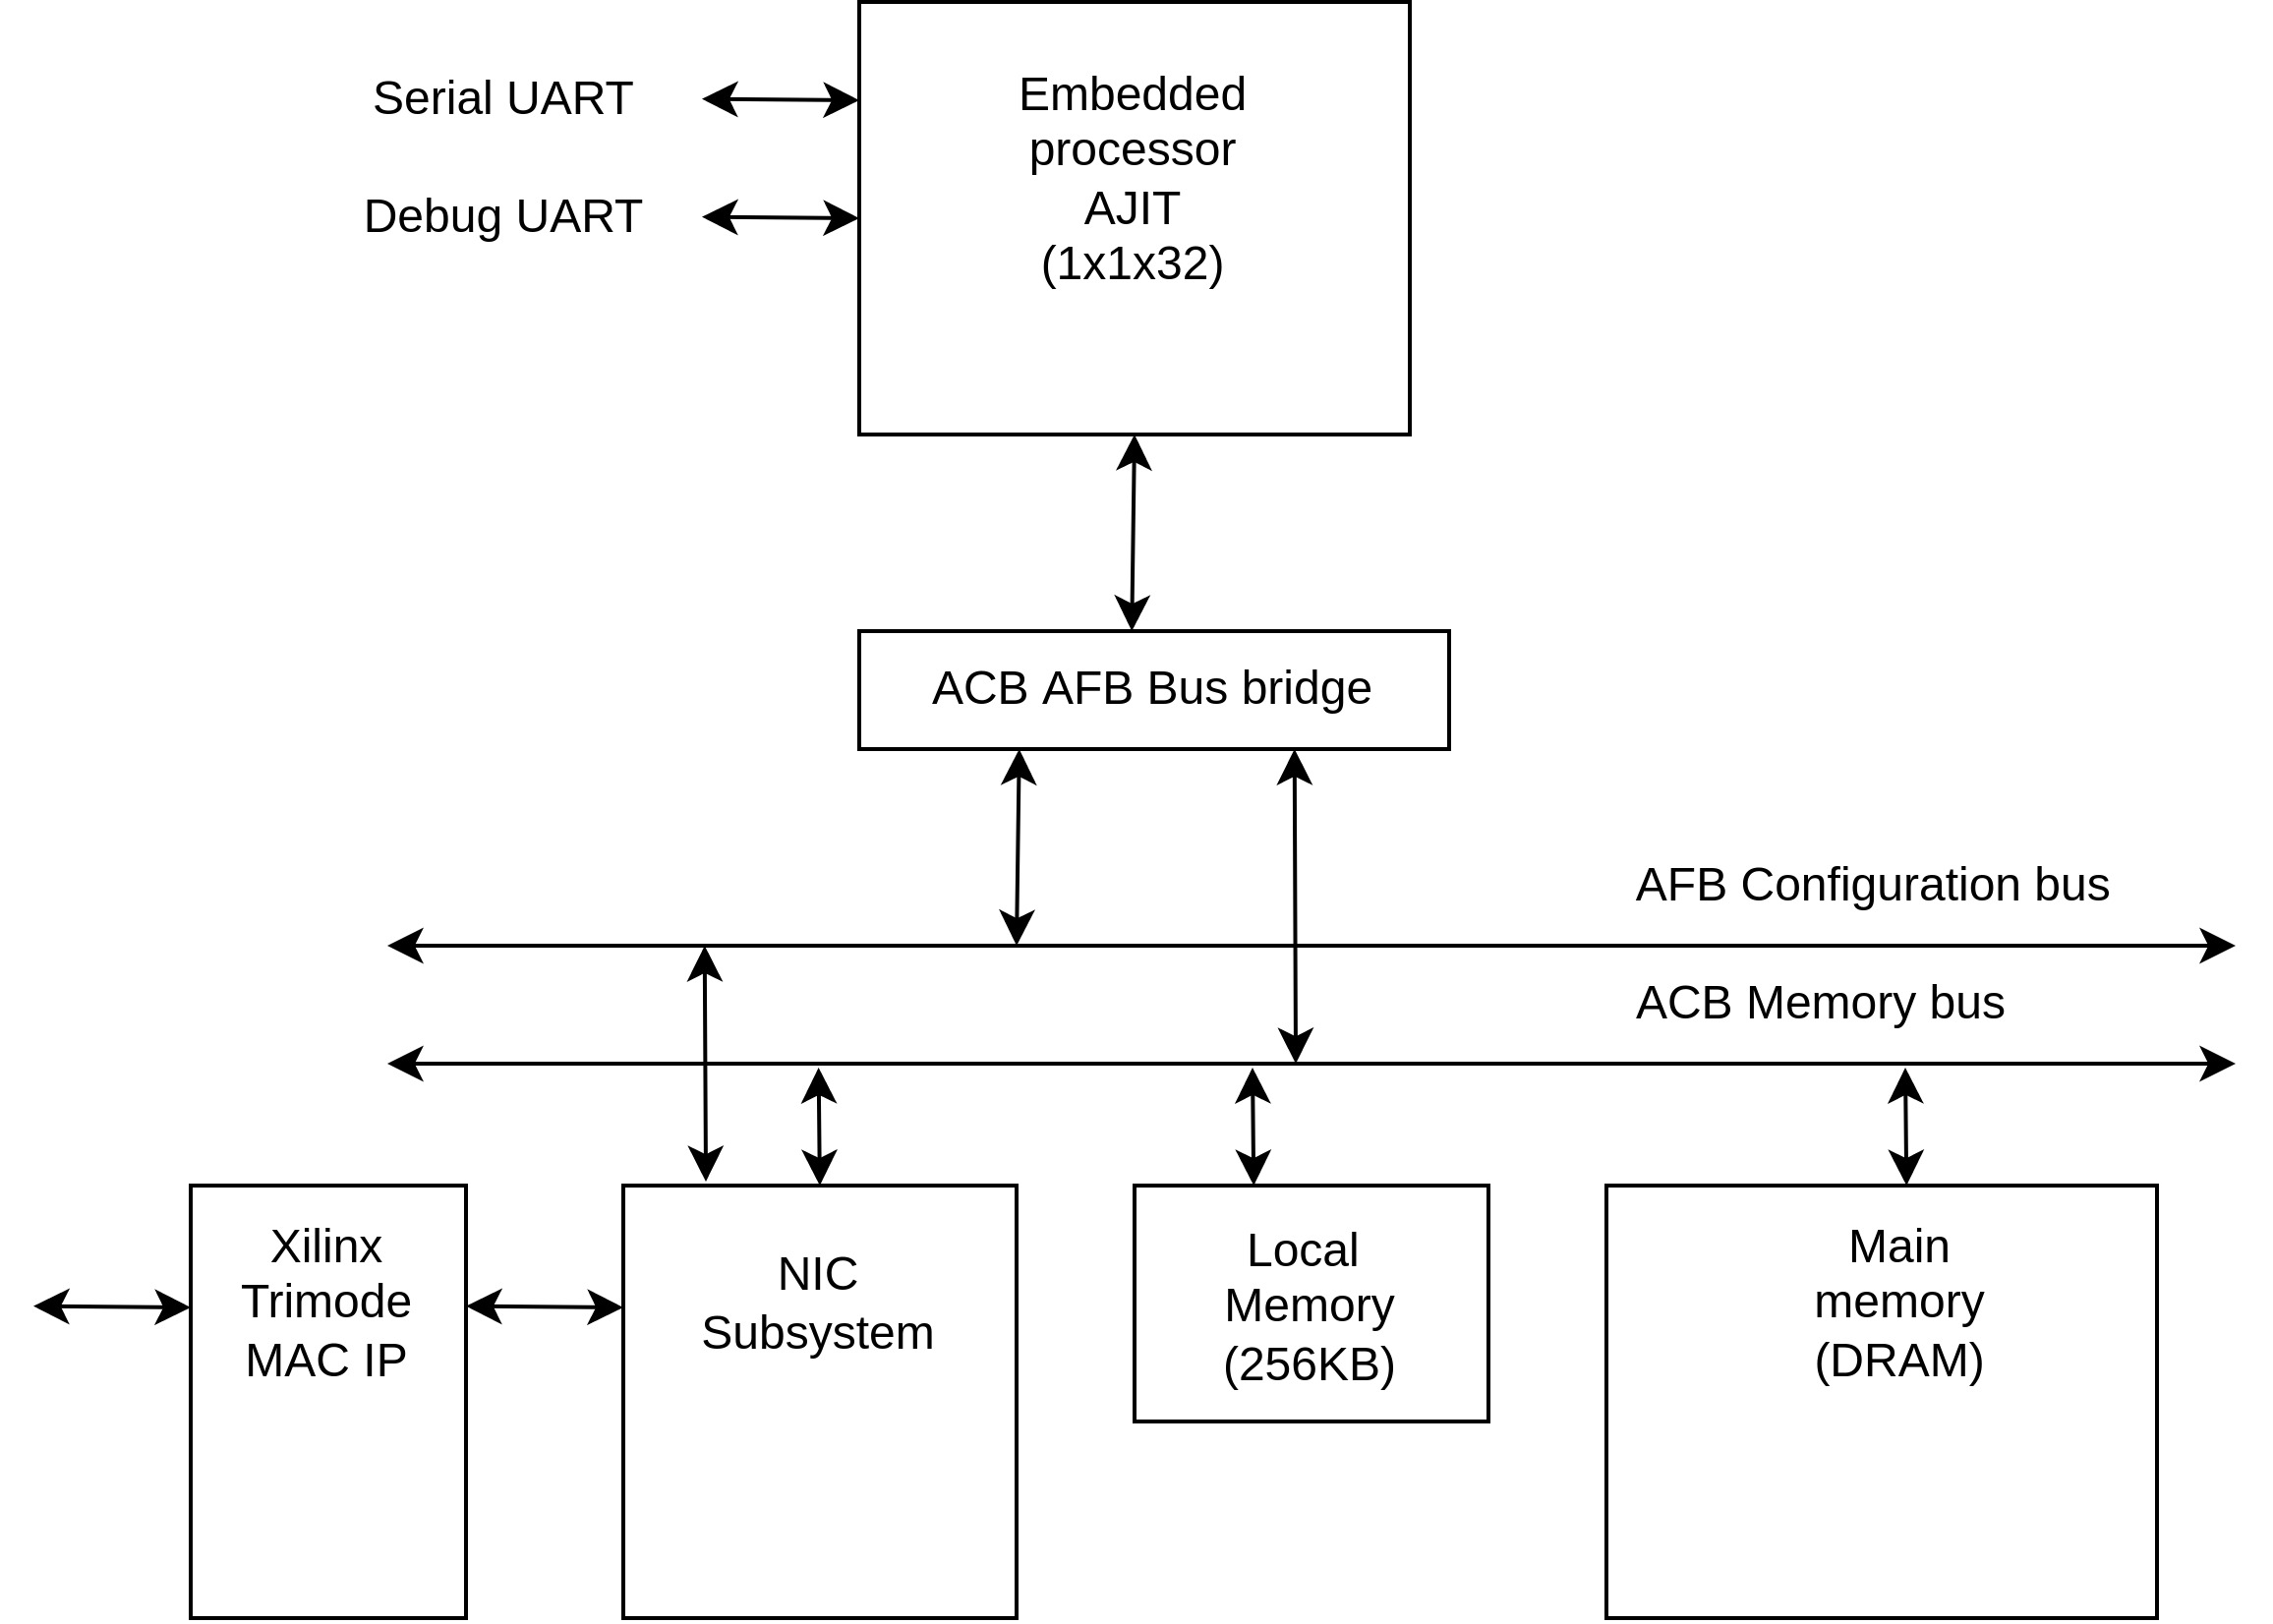
\includegraphics[width=14cm]{../figures/ACB_SRAM_arch.jpg}
			\caption{NIC and processor sharing a fast local packet memory of 256KB}
			\label{fig:NIC-Proc-top-level2}
		\end{figure}
\section{Performance Characterization of Optimization A}
The SoC was implemented and validated on KC-705 FPGA.
The performance of the SoC was characterized using two applications, namely the standard Ping application and the Network content cache application. Both the applications were executed in a bare-metal environment using an open-source TCP/IP stack, lwIP(lightweight IP), which was ported for the AJIT processor and custom-designed NIC. 

\subsection{Average round trip time (RTT)}
To measure the average RTT, ICMP request packets were generated using the standard ping command from a Linux terminal on a host machine and sent to the SoC on the FPGA. The processor core was running at 80MHz, the NIC subsystem was operating at 125MHz with a 1Gbps Ethernet link, and the lwIP TCP/IP stack generated ICMP response packets.

\begin{table*}[h!]
\caption{Avg RTT time and Data rate achieved for different  packet sizes}
\begin{center}
\begin{tabular}{|c|c|}

\hline
\textbf{Packet size(bytes)} & \textbf{Average RTT (us)}  \\
\hline
64 & 216    \\
\hline
128 & 261   \\
\hline
256 & 288   \\
\hline
512 & 313   \\
\hline
1024 & 337   \\
\hline
\end{tabular}
\label{table_dataRate1}
\end{center}
\end{table*}



\newpage
\subsection{Network Content Caching application}
In this application, the SoC setup is deployed on the FPGA, where both the lwIP server and client are running. Two hosts, A and B, are operating on the host side (PC or laptop). Host A pre-populates the cache (DRAM) with frequently needed data via a TCP connection. When Host B requests data from Host A, Host A sends a "forward" command to the lwIP server on the FPGA, including Host B's IP address and port number. The lwIP server then forwards the data to Host B using a UDP connection. The data transmission speeds for populating the "cache" on the FPGA by Host A and forwarding data from the "cache" on the FPGA to Host B are reported below.
\begin{enumerate}
    \item Host A(on PC) to Controller (On FPGA): 28.77 Mbps
    \item Controller (On FPGA) to Host B (on PC) :16.22 Mbps
\end{enumerate}

(\textbf{Application is described in more detail in appendix B})


%%%%%%%%%%%%%%%%%%%%%%%%%%%%%%%%%%%%%%%%%%%%%%%%%%%%%%%%%%%%%%%%%%%%%%%%%%%%%%%%%%%%%%%



\section{Optimization B: Using an L2 cache in NIC and the processor access path to main memory (DRAM)}
The proposed architecture introduces a novel approach to accessing descriptor ring structures and packet buffers, moving away from direct access in slower main memory (DRAM). Instead, these critical components are accessed through an inclusive write-back L2 cache shared between the Network Interface Card (NIC) and the processor. This architectural choice aims to optimize data access speeds and enhance overall system performance.

By utilizing an inclusive write-back L2 cache, the architecture leverages the benefits of caching mechanisms to improve access latency for descriptor rings and packet buffers. This shared cache design ensures that frequently accessed data remains readily available to both the NIC and the processor, reducing the need for repeated accesses to the slower DRAM.

Accessing descriptor ring structures and packet buffers through the L2 cache streamlines data retrieval operations. The cache's inclusive nature ensures that data accessed by one entity (either the NIC or the processor) is also available in the cache for subsequent accesses by the other entity. This approach minimizes latency and enhances the responsiveness of the system to incoming and outgoing network traffic.
The architecture is shown below.

	\begin{figure}[h]
			\centering
			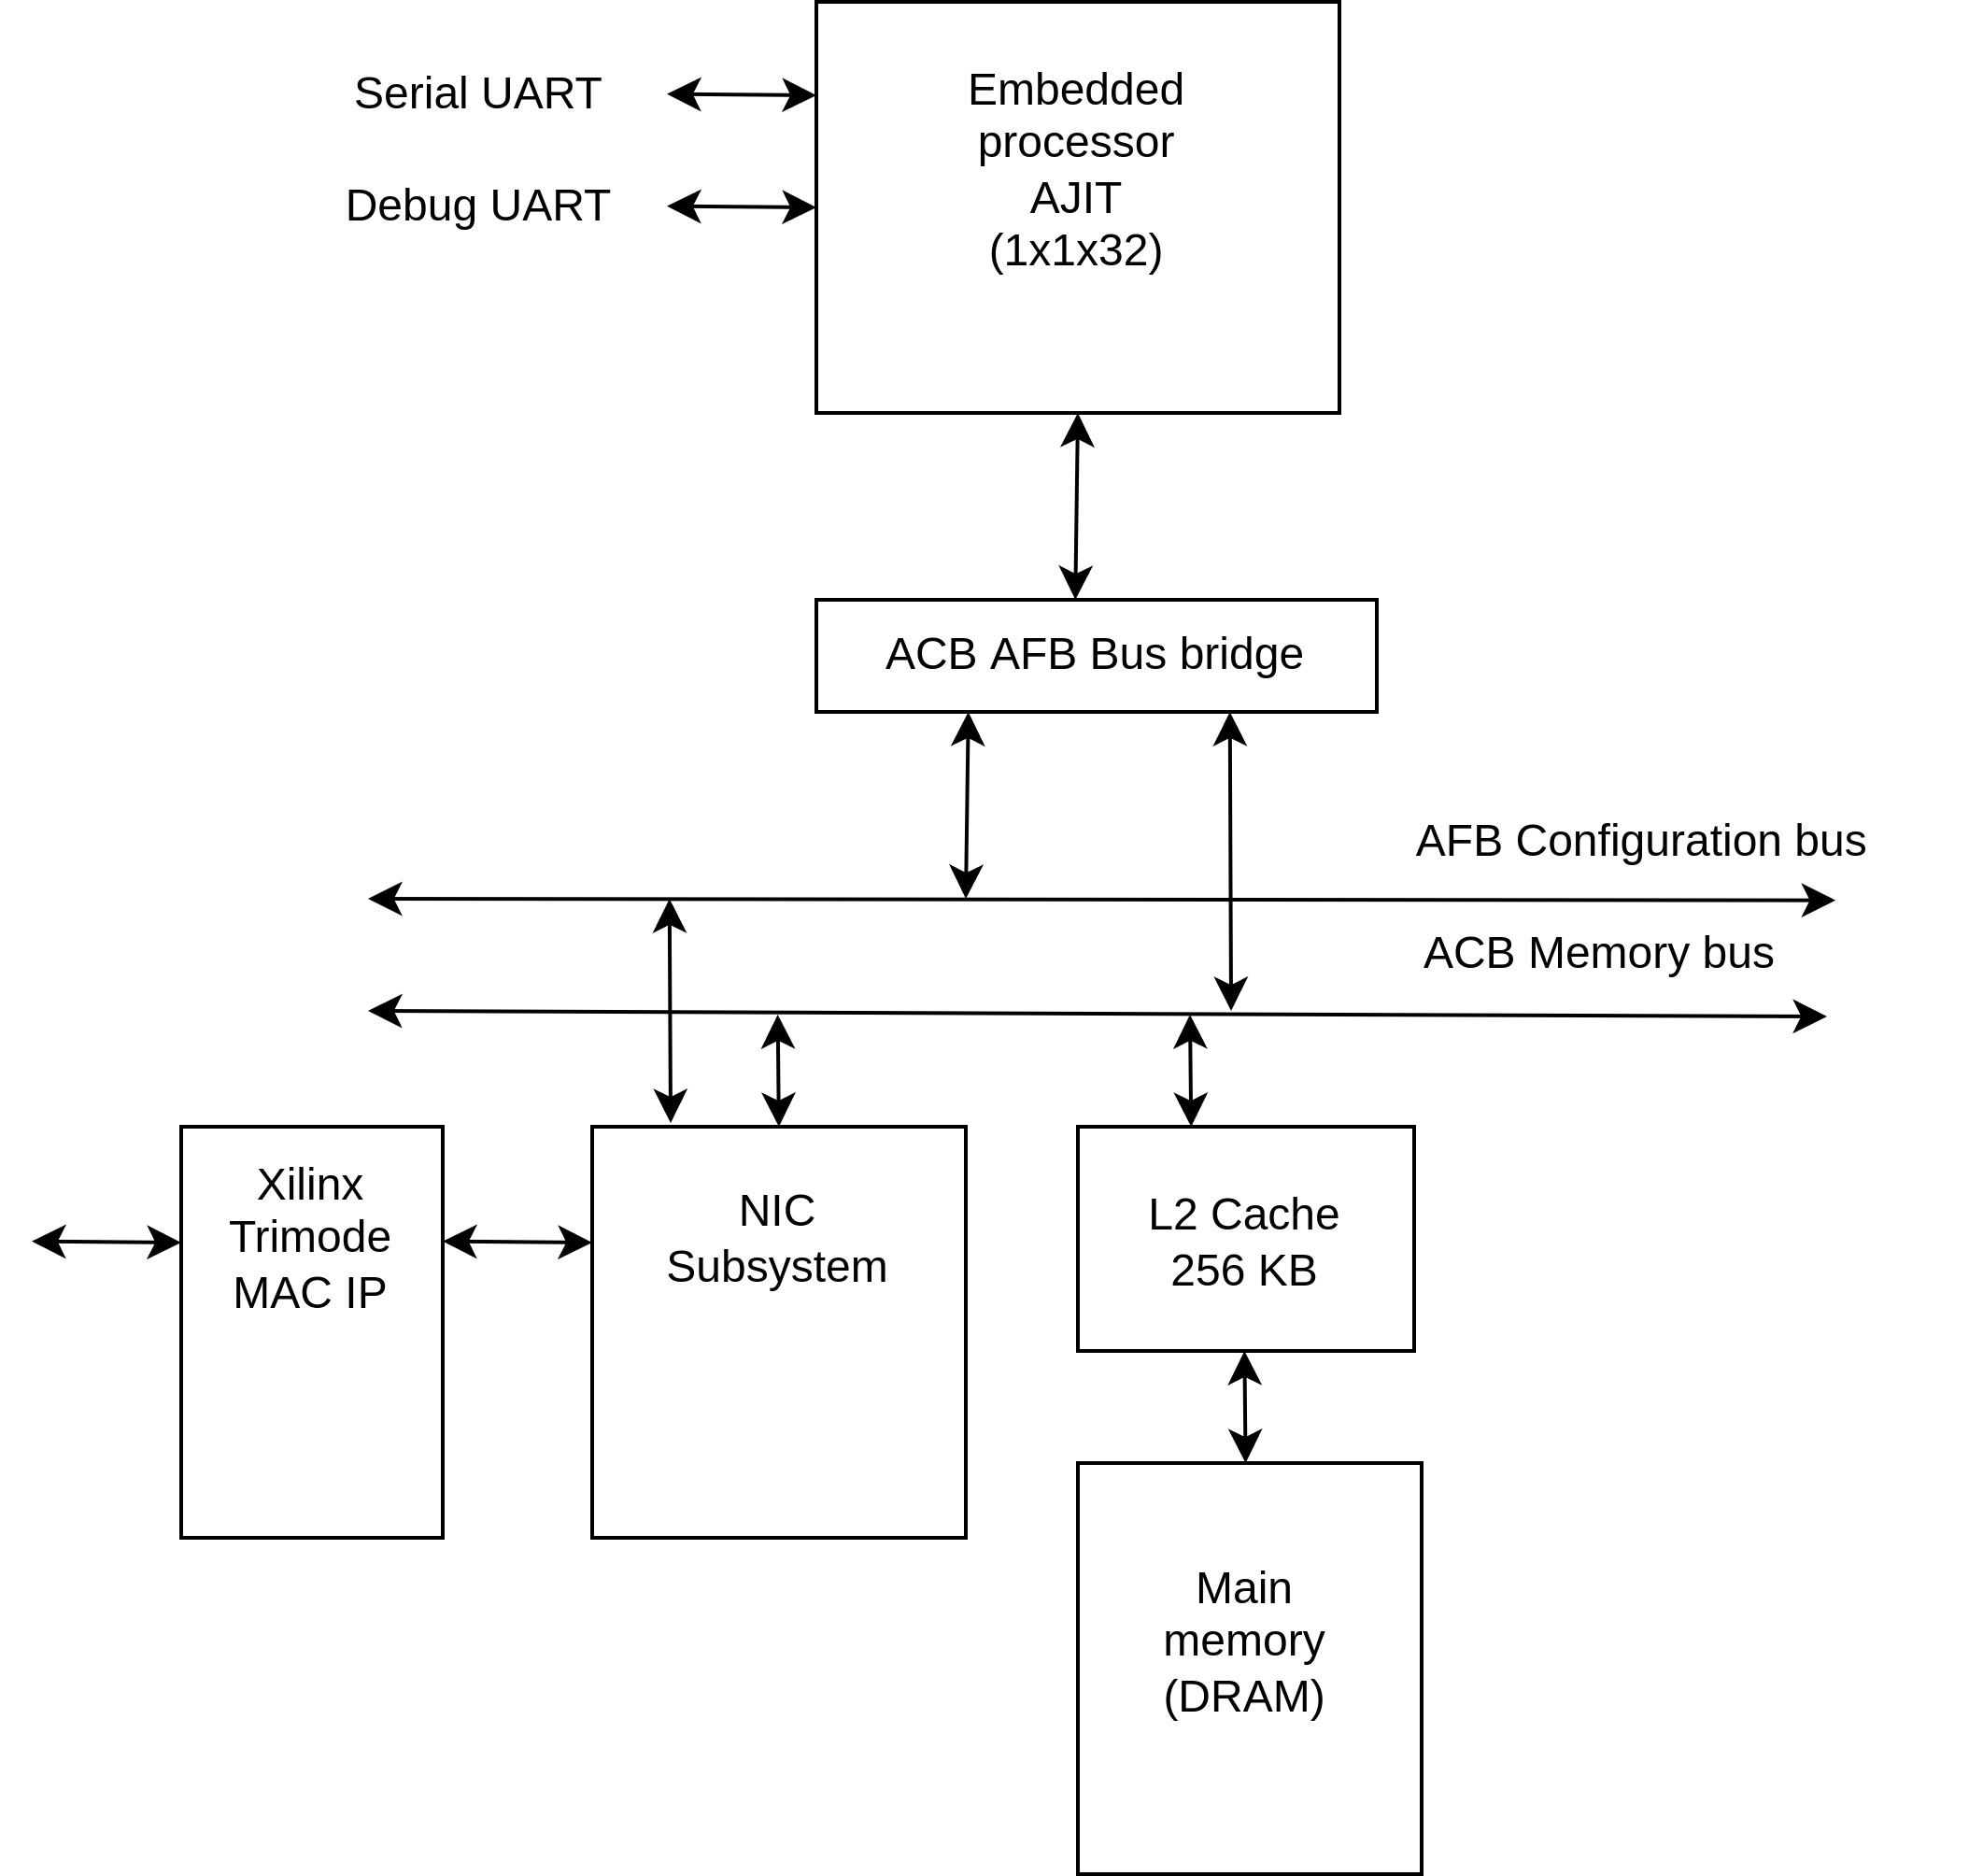
\includegraphics[width=12cm]{../figures/L2Cache_arch.jpg}
			\caption{NIC and processor access main memory via L2 cache}
			\label{fig:NIC-Proc-top-level3}
		\end{figure}
\section{Performance Characterization of Optimization B}
The SoC was implemented and validated on KC-705 FPGA.
The performance of the SoC was characterized using two applications, namely the standard Ping application and the Network content cache application. Both the applications were executed in a bare-metal environment using an open-source TCP/IP stack, lwIP(lightweight IP), which was ported for the AJIT processor and custom-designed NIC. 

\subsection{Average round trip time (RTT)}
To measure the average RTT, ICMP request packets were generated using the standard ping command from a Linux terminal on a host machine and sent to the SoC on the FPGA. The processor core was running at 80MHz, the NIC subsystem was operating at 125MHz with a 1Gbps Ethernet link, and the lwIP TCP/IP stack generated ICMP response packets.

\begin{table*}[h!]
\caption{Avg RTT time and Data rate achieved for different  packet sizes}
\begin{center}
\begin{tabular}{|c|c|}

\hline
\textbf{Packet size(bytes)} & \textbf{Average RTT (us)}  \\
\hline
64 & 245    \\
\hline
128 & 288   \\
\hline
256 & 322   \\
\hline
512 & 350   \\
\hline
1024 & 371   \\
\hline
\end{tabular}
\label{table_dataRate2}
\end{center}
\end{table*}



\newpage
\subsection{Network Content Caching application}
In this application, the SoC setup is deployed on the FPGA, where both the lwIP server and client are running. Two hosts, A and B, are operating on the host side (PC or laptop). Host A pre-populates the cache (DRAM) with frequently needed data via a TCP connection. When Host B requests data from Host A, Host A sends a "forward" command to the lwIP server on the FPGA, including Host B's IP address and port number. The lwIP server then forwards the data to Host B using a UDP connection. The data transmission speeds for populating the "cache" on the FPGA by Host A and forwarding data from the "cache" on the FPGA to Host B are reported below.
\begin{enumerate}
    \item Host A(on PC) to Controller (On FPGA): 27 Mbps
    \item Controller (On FPGA) to Host B (on PC) : 14.22 Mbps
\end{enumerate}
(\textbf{Application is described in more detail in appendix B})
%%%%%%%%%%%%%%%%%%%%%%%%%%%%%%%%%%%%%%%%%%%%%%%%%%%%%%%%%%%%%%%%%%%%%%%%

\newpage
\chapter{Conclusion \& Future Work} \label{4}
\rule[10pt]{\linewidth}{3pt}	

\section {Conclusion}
A comparative analysis of three architectures—the Baseline architecture, Optimization A where the Processor and NIC share a fast local packet memory, and Optimization B where the Processor and NIC access main memory via L2 Cache—reveals that Optimization A yields a performance gain of 34.5\%, while Optimization B results in an 18.3\% improvement. Therefore, the Optimization A architecture is recommended for designing the memory subsystem to ensure sufficient fast buffering for packets in the data plane. \\ 

From Table 4.1 and Figure 4.1, we can observe that to transmit an additional 512 bytes or 4096 bits, on average, 21.67 us is required. Therefore we can achieve a throughput of \textbf{378 Mbps}, with the current setup. One can also observe from the Y-intercept
the software overhead of about 152 us. \\

Further optimization opportunities can be explored by enhancing the architecture to offload additional computational tasks to the NIC. This approach could streamline processing within the SoC, leveraging the NIC's capabilities to handle specific tasks more efficiently.

\begin{figure}[h]
			\centering
			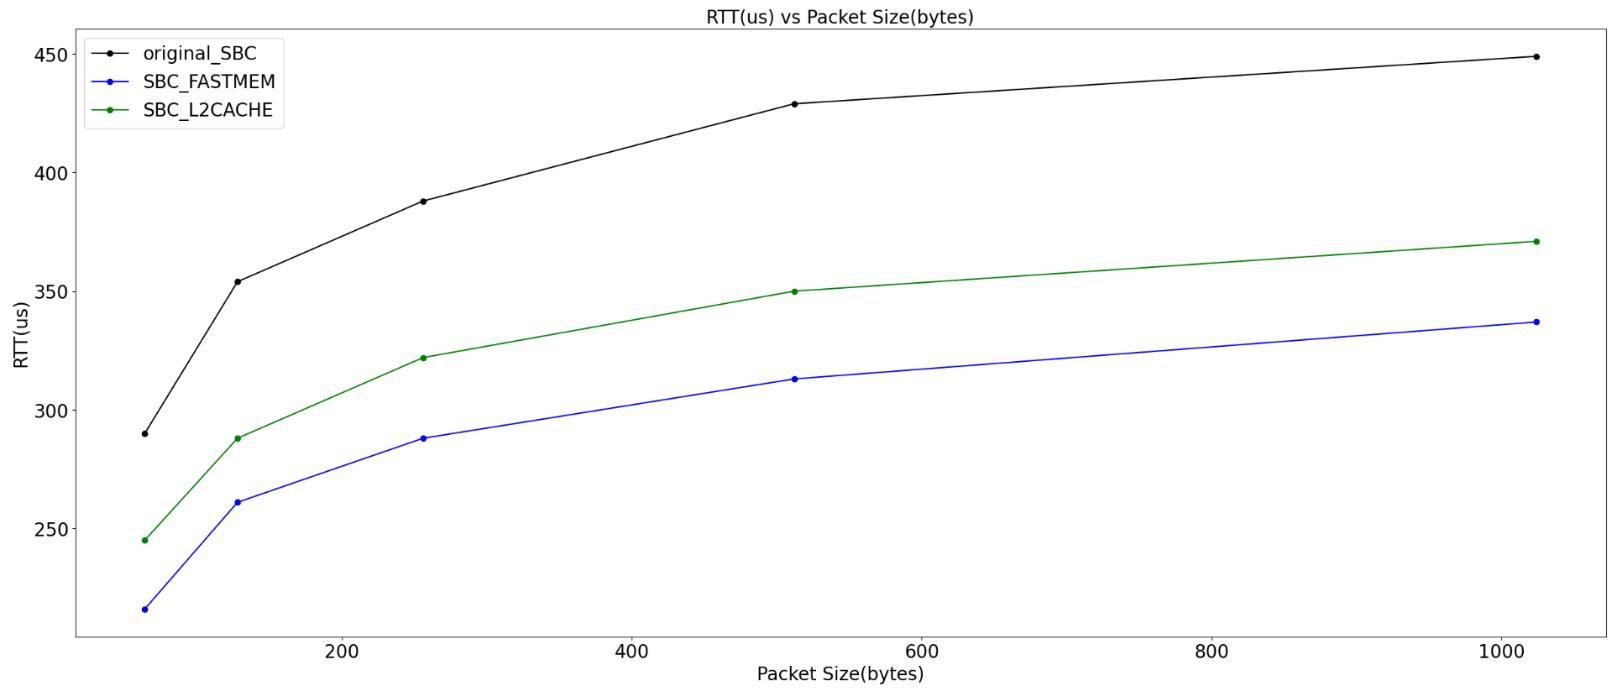
\includegraphics[width=16cm]{../figures/final123.jpg}
			\caption{Round Trip Time vs Packet Size}
			\label{fig:NIC-Proc-top-level4}
		\end{figure}



\begin{table*}[h!]
\caption{Avg RTT time and for different  packet sizes and different architectures}
\begin{center}
\begin{tabular}{|c|c|c|c|}

\hline
\textbf{Packet (bytes)}
& \textbf{RTT (us) Baseline} 
& \textbf{RTT (us) Packet memory}  
& \textbf{RTT (us) L2 Cache}  \\
\hline
64 & 290 & 216   &  245 \\
\hline
128 & 354 &  261  & 288  \\
\hline
256 & 388 &  288  & 322  \\
\hline
512 & 429  &  313  & 350 \\
\hline
1024 & 449 &  337  &  371  \\
\hline
\end{tabular}
\label{table_dataRate3}
\end{center}
\end{table*}


\begin{table*}[h!]
\caption{Uplink and Downlink speed (Mbps) for network caching application}
\begin{center}
\begin{tabular}{|c|c|c|c|}

\hline
\textbf{}
& \textbf{Data rate Baseline} 
& \textbf{Data rate Packet memory}  
& \textbf{Data rate L2 Cache}  \\
\hline
Host A To FPGA & 23.7 & 28.77   &  27.12 \\
\hline
FPGA To Host B & 13.43 &  16.22  & 14.22  \\
\hline

\hline
\end{tabular}
\label{table_dataRate4}
\end{center}
\end{table*}


\newpage
\section{Future Work}
\begin{enumerate}
    \item Various computational tasks can be further optimized by offloading them to the NIC, such as TCP offloads and checksum generation.
    \item In Optimization A, enhancing packet handling by directly transferring packets to main memory using DMA instead of the current "memcpy()" function.
    \item Scaling the SoC to incorporate multiple cores, allowing for separation of control plane management in one core and data plane operations in others.
   
\end{enumerate}






%%%%%%%%%%%%%%%%%%%%%%%%%%%%%%%%%%%%%%%%%%%%%%%%%%%%%%%%%%%%%%%%%%%%%%%%%%%%%%%%%%%%%%%
\begin{appendices}


\chapter{ Standard NIC (Network Interface Controller) Design - By MPD}

\rule[10pt]{\linewidth}{3pt}

This chapter focuses on the design of the Network Interface Controller (NIC) for the AJIT processor-based System-on-Chip (SoC). The NIC is crucial for providing network connectivity and communication capabilities within the SoC. The design process involves various components and considerations, such as network protocol support, data packet handling, memory management, and interfacing with the AJIT processor. This chapter aims to offer a comprehensive overview of the NIC design, detailing the key components and their interconnections. It also examines the challenges faced during the design phase and discusses the solutions and design choices implemented to address them.
	
	\section{Design decisions}
		Before directly jumping on NIC design let's take a look at the necessary design decisions made. The NIC will receive packet data from MAC
		which will be stored in memory. The processor will need to allocate this memory and provide that information to NIC. This overall needs to
		3 main interfaces to NIC. Figure~\ref{fig:NIC-Proc-top-level5} shows all the interfaces.We examine each interface in detail.	

		\begin{figure}[h]
			\centering
			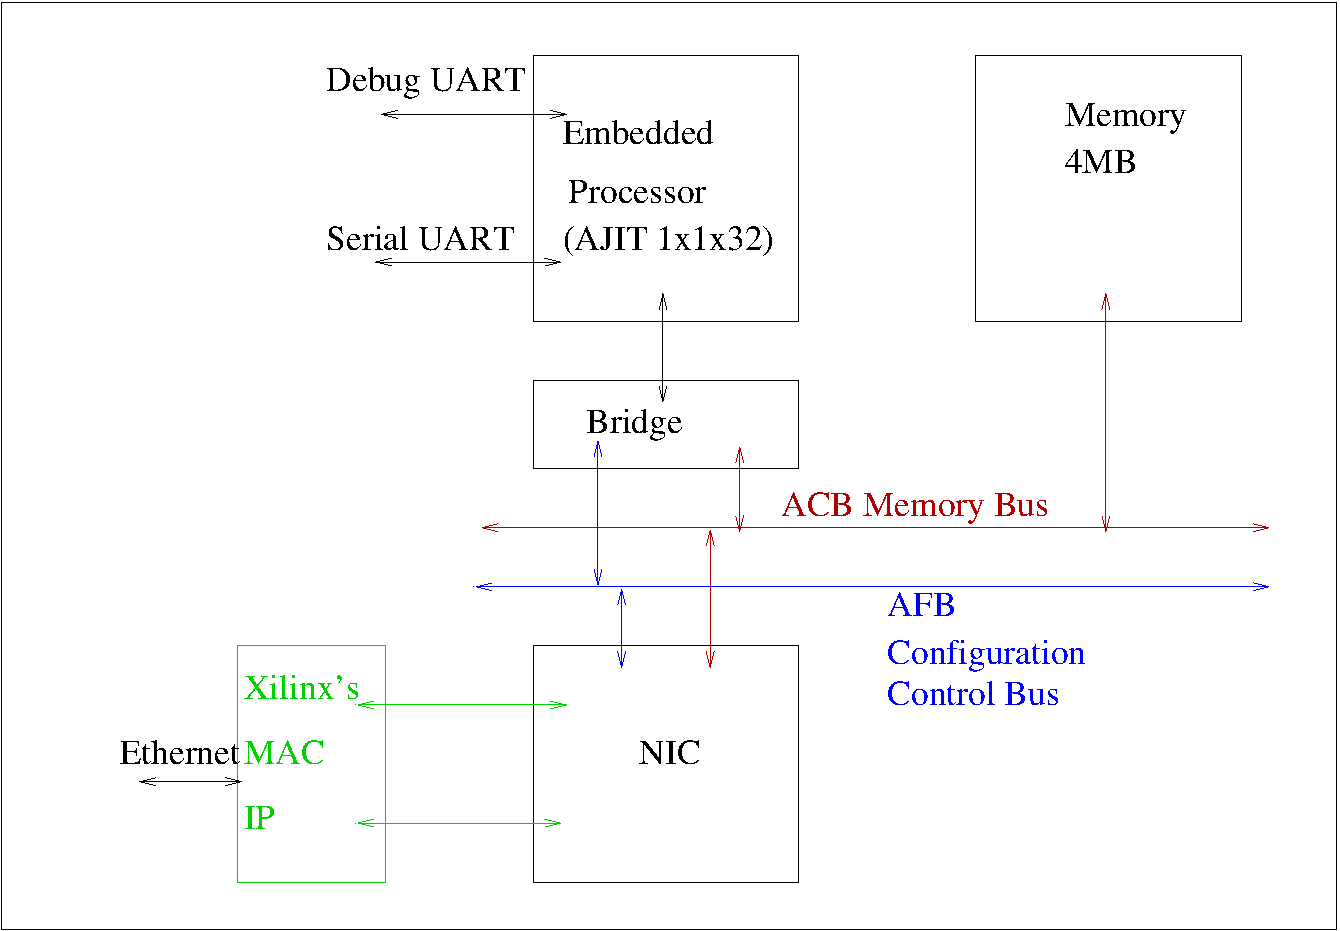
\includegraphics[width=12cm]{../figures/top_level_for_interfaces.pdf}
			\caption{Top level with Interfaces}
			\label{fig:NIC-Proc-top-level6}
		\end{figure}




		\subsection{NIC-MAC interface}
			NIC to MAC interface will used by NIC for receiving and transmitting packets from MAC. The memory which will be used is provided 8 bytes per request.
			So this interface is kept 73(64 bit data + 9 bit control) bits. The bit mapping is shown in table~\ref{tab:NIC-MAC-interface}.
				\begin{table}[!htbp]
					\centering
					\begin{tabular}{ccl}
						\hline
						\textbf{Signal Name} & \textbf{Location} &\textbf{Signal Description}  \\ \hline
						\multirow{2}{*}{\textit{tlast}}	& \multirow{2}{*}{[72:72]}	& The \textit{tlast} becomes `1' if the 64 bit chunk is last\\
										& 				& chunk of packet.\\ \hline
						\textit{tdata}   		& [71: 8] 			& The \textit{tdata} is actual packet data chunk.\\ \hline
						\multirow{3}{*}{\textit{tkeep}}	& \multirow{3}{*}{[ 7: 0]}	& The \textit{tkeep} is 8 bit field, each bit is mapped\\
										&				& to 8 bytes of data. If any bit is `1' then\\
										& 				& corresponding byte in data is valid else not.\\ \hline 
					\end{tabular}
					\caption{NIC-MAC interface description}
					\label{tab:NIC-MAC-interface}
				\end{table}
			The same interface will be used for both reception and transmission of packets.

		\subsection{NIC-Memory interface}
			The NIC-Memory interface is required for storeing and loading packets to and from memory. Already developed ACB(AJIT Core Bus) protocol will be used for this.
                        The protocol consists of two interfaces,
			\begin{enumerate}
				\item ACB Requeuest : Requests from NIC to store and load the packet will be sent through this interface. see table~\ref{tab:NIC-Memory-interface-req} for bit mapping.
				\item ACB Response : Response generated by memory to the request will be sent back to NIC on this interface. see table~\ref{tab:Memory-NIC-interface-resp} for bit mapping.
			\end{enumerate}

				\begin{table}[!htbp]
					\centering
					\begin{tabular}{ccl}
						\hline
						\textbf{Signal Name} 			& \textbf{Location} 		&\textbf{Signal Description}  \\ \hline
						\multirow{2}{*}{\textit{lock}}		& \multirow{2}{*}{[109:109]}	& Lock bit, if set to `1' by a master then\\
											&				& other master's don't get access to Memory.\\ \hline
						\multirow{2}{*}{\textit{read/write\_bar}}& \multirow{2}{*}{[108:108]}	& If `1', the request is read request,\\ 
											& 				& if `0', the request is write request.\\ \hline
						\multirow{3}{*}{\textit{byte\_mask}}	& \multirow{3}{*}{[ 107: 100]}	& The \textit{byte\_mask} is 8 bit field, each bit is mapped\\
											&				& to 8 bytes of data. If any bit is `1' then\\
											& 				& corresponding byte in data is valid else not.\\ \hline 
						\multirow{2}{*}{\textit{address}}   	& \multirow{2}{*}{[99:64]} 	& The addres(byte) where read/write should\\ 
											&				& be performed.\\ \hline
						\textit{write\_data}   			& [63: 0] 			& Data to be written.\\ \hline
					\end{tabular}
					\caption{NIC - Memory interface description}
					\label{tab:NIC-Memory-interface-req}
				\end{table}

				\begin{table}[!htbp]
					\centering
					\begin{tabular}{ccl}
						\hline
						\textbf{Signal Name} 		& \textbf{Location} 		&\textbf{Signal Description}  \\ \hline
						\textit{err}			& [64:64]			& Value `1' indicates errored response.\\\hline
						\textit{data}   		& [63: 0] 			& Contains read data if the req. was read req.\\ \hline
					\end{tabular}
					\caption{Memory - NIC interface description}
					\label{tab:Memory-NIC-interface-resp}
				\end{table}
			
		\subsection{NIC-Processor interface} \label{AFB}
			This will be more of a control interface. Processor will allocate the memory space for packet storage and provide thaat info to NIC using this interface.
			NIC will have registers inside which will written by the processor using this interface. For further information see section~\ref{subsec:NIC_REG}. An already developed
			AFB(AJIT FIFO Bus) protocol will be used for this. This AFB protocol also has two interfaces like ACB protocol only the address width is half.

			\begin{enumerate}
				\item AFB Requeuest : Requests from Processor to write or read the NIC reg will be sent through this interface. 
				\item AFB Response : Response generated by NIC to the request will be sent back to Processor on this interface.
			\end{enumerate}

				\begin{table}[h]
					\centering
					\begin{tabular}{ccl}
						\hline
						\textbf{Signal Name} 			& \textbf{Location} 		&{c}\textbf{Signal Description}  \\ \hline
						\multirow{2}{*}{\textit{lock}}		& \multirow{2}{*}{[73:73]}	& Lock bit, if set to `1' by a master then\\
											&				& other master's don't get access to Memory.\\ \hline
						\multirow{2}{*}{\textit{read/write\_bar}}& \multirow{2}{*}{[72:72]}	& If `1', the request is read request,\\ 
											& 				& if `0', the request is write request.\\ \hline
						\multirow{3}{*}{\textit{byte\_mask}}	& \multirow{3}{*}{[ 71: 68]}	& The \textit{byte\_mask} is 4 bit field, each bit is mapped\\
											&				& to 4 bytes of data. If any bit is `1' then\\
											& 				& corresponding byte in data is valid else not.\\ \hline 
						\multirow{2}{*}{\textit{address}}   	& \multirow{2}{*}{[67:32]} 	& The addres(byte) where read/write should\\ 
											&				& be performed.\\ \hline
						\textit{write\_data}   			& [31: 0] 			& Data to be written.\\ \hline
					\end{tabular}
					\caption{Processor - NIC interface description}
					\label{tab:Proc-NIC-interface-req}
				\end{table}

				\begin{table}[!htbp]
					\centering
					\begin{tabular}{ccl}
						\hline
						\textbf{Signal Name} 		& \textbf{Location} 		&\textbf{Signal Description}  \\ \hline
						\textit{err}			& [32:32]			& Value `1' indicates errored response.\\\hline
						\textit{data}   		& [31: 0] 			& Contains read data if the req. was read req.\\ \hline
					\end{tabular}
					\caption{ NIC - Procesor interface description}
					\label{tab:NIC-Proc-interface-resp1}
				\end{table}

	
	\section{Interface data structures}

		The interface data structures used in the NIC design consist of three queues: the free\_queue, rx\_queue, and tx\_queue.


		%\begin{figure}[h]
		%	\centering
		%	\includegraphics[width=8cm]{./figures/queues.pdf}
		%	\caption{Add this fig which will have all queue interfaces}
		%	\label{fig:queue_interface}
		%\end{figure}


	\begin{itemize}

 
		\item \textbf{receive\_free\_queue}: This queue holds the addresses of free buffers that are available for storing/receiving packets. The processor initially assigns a set of buffers and pushes their physical addresses into this free queue. NIC (HW side) pops a free buffer pointer from this free queue, and
	writes data into the buffer, and pushes the free 
        buffer to the receive queue. The processor (SW side) pops the buffer from the receive queue, processes the packet, and pushes the buffer pointer back to the free queue for further reception of packets.\\

        \item \textbf{transmit\_free\_queue}: This queue holds the addresses of free buffers that are available for transmitting the packets. The processor initially assigns a set of buffers and pushes their physical addresses into this free queue. Processor(SW side) pops a free buffer pointer from this free queue, and
	writes data into the buffer, and pushes the free 
        buffer to the transmit queue.
	NIC (HW side) pops the buffer from the transmit queue, transmits it, and pushes the buffer pointer back to the free queue, for further transmission of packets. \\

		\item \textbf{rx\_queue}: The rx\_queue contents are pushed by the NIC and popped by the processor. It holds the addresses of buffers that currently contain active packets. When the NIC receives a packet, it stores the packet in a buffer and pushes the address of that buffer into the rx\_queue. This allows the processor to identify the buffers with active packets that are ready for processing. \\

		\item \textbf{tx\_queue}: The tx\_queue contents are pushed by the processor and popped by the NIC. Once the processor has finished processing a packet, it pushes the address of the processed packet buffer into the tx\_queue. The NIC monitors the tx\_queue and retrieves the buffer addresses from it to send the packets out over the network.\\
	\end{itemize}

These queues enable efficient coordination and communication between the processor and the NIC, ensuring the proper handling and processing of packets.

To ensure synchronization and prevent conflicts during access to these queues, a locking mechanism is implemented. The locking mechanism utilizes atomic operations, which guarantee thread-safe access and modifications to the queues. This ensures that only one entity can perform push and pop operations on the queues at a given time, preventing simultaneous modifications and preserving the integrity of the queue data.


At startup, the processor initializes the queues by allocating memory for them and configuring their initial state. The addresses of these queues are then communicated to the NIC by writing to specific NIC registers. This process allows the NIC to access and manipulate the queues effectively during runtime. 

		%These are all interface decisions taken lets now move on to NIC design. Let's see the NIC registers now.

	\section{Network Interface Controller}
		


		\subsection{Register File Map} \label{subsec:NIC_REG}
				The NIC (Network Interface Controller) registers are specific memory locations within the NIC that are used for configuration, control, and status monitoring purposes. These registers allow communication between the processor and the NIC, enabling the processor to control and monitor NIC. The NIC registers provide a standardized interface for the processor to interact with the NIC and perform tasks such as enabling or disabling the NIC, setting queue address and monitoring the status of data transmission and reception. See table~\ref{tab:NIC_REG} for description of NIC registers.

			\begin{table}[h!]
				\centering
				\begin{tabular}{|c|c|c|}
					\hline
					Reg. ID& Address offset & Description  \\ \hline
					
				
                         8  & 0xC0   & RxQ server 0  physical address[35:32]      \\ \hline
                         9  & 0x20   & RxQ server 0  physical address[31:0]  \\ \hline
                         10  & 0x24   & RxQ server 0  lock physical address[35:32]  \\ \hline
					11  & 0x2C   & RxQ server 0  lock physical address[31:0]  \\ \hline
					12  & 0x30   & RxQ server 0 buffer physical address[35:32] \\ \hline
                        13  & 0x34   & RxQ server 0 buffer physical address[31:0] \\ \hline

                        128  & 0x400   & TxQ server 0  physical address[35:32]      \\ \hline
                         129  & 0x404   & TxQ server 0  physical address[31:0]  \\ \hline
                         130  & 0x408   & TxQ server 0  lock physical address[35:32]  \\ \hline
					131  & 0x40C   & TxQ server 0  lock physical address[31:0]  \\ \hline
					132  & 0x410   & TxQ server 0 buffer physical address[35:32] \\ \hline
                        133  & 0x414   & TxQ server 0 buffer physical address[31:0] \\ \hline

                       200  & 0x320   & Base address of free Queue Tx  [35:4]      \\ \hline
                         201  & 0x324    & Base address of free Queue Tx [31:0]  \\ \hline
                         202  & 0x328   & Lock address for free Queue Tx [35:4]  \\ \hline
					203  & 0x32C   & Lock address for free Queue Tx [31:0]  \\ \hline
					204  & 0x330   & Buffer address for free Queue Tx [35:4] \\ \hline
                        205  & 0x334   & Buffer address for free Queue Tx [31:0] \\ \hline





                          213  & 0x350   & Base address of free Queue Tx  [35:4]      \\ \hline
                         214  & 0x354    & Base address of free Queue Tx [31:0]  \\ \hline
                         215  & 0x358   & Lock address for free Queue Tx [35:4]  \\ \hline
					216  & 0x35C   & Lock address for free Queue Tx [31:0]  \\ \hline
					217  & 0x360   & Buffer address for free Queue Tx [35:4] \\ \hline
                        218  & 0x364   & Buffer address for free Queue Tx [31:0] \\ \hline


                        
                       
				\end{tabular}
				\caption{NIC registers map}
				\label{tab:NIC_REG}
			\end{table}



		\subsection{Receive Enigne}
				The receive engine daemon is responsible for the storage of packets coming from the parser. It receives the parsed packet information from the parser daemon and interacts with the processor to ensure the proper handling of received packets. The receive engine daemon uses the free\_queue, to get an empty buffer address to store the active packets in buffers.
			Then uses rx\_queue to provide their(buffer's) addresses to the processor for processing. 
		\subsection{Transmit Engine}
				The transmit engine daemon focuses on transmitting processed packets from the processor to the external network. It receives the addresses of processed packet buffers from the processor via the tx\_queue and sends the corresponding packets out through the Ethernet interface. The transmit engine daemon monitors the tx\_queue and retrieves the buffer addresses to facilitate efficient packet transmission. The daemon also pushes free\_queue with the address of buffers which is sent out. This allows the reuse of buffers. 
			
		\subsection{Nic register Access}
				The NIC register access daemon provides the necessary interface for the NIC to read from and write to its internal registers. These registers store critical information for the proper functioning of the NIC, including configuration settings, status flags, and other control parameters. The NIC register access daemon ensures that the processor can interact with these registers and modify them as needed to configure and manage the NIC's behavior.
		\begin{table}[!htbp]
					\centering
					\begin{tabular}{ccl}
						\hline
						\textbf{Signal Name} 			& \textbf{Location} 		&{c}\textbf{Signal Description}  \\ \hline
						\multirow{2}{*}{\textit{read/write\_bar}}& \multirow{2}{*}{[42:42]}	& if `1', the request is read request,\\ 
											& 				& if `0', the request is write request.\\ \hline
						\multirow{3}{*}{\textit{byte\_mask}}	& \multirow{3}{*}{[ 41: 38]}	& \textit{byte\_mask} is 4 bit field, each bit is mapped\\
											&				& to 4 bytes of data. if any bit is `1' then\\
											& 				& corresponding byte in data is valid else not.\\ \hline 
						\multirow{2}{*}{\textit{reg\_index}}   	& \multirow{2}{*}{[37:32]} 	& index of register to which read/write should\\ 
											&				& be performed.\\ \hline
						\textit{write\_data}   			& [31: 0] 			& Data to be written.\\ \hline
					\end{tabular}
					\caption{NIC to Register file interface description}
					\label{tab:NIC-Reg-interface-req}
				\end{table}

				\begin{table}[!htbp]
					\centering
					\begin{tabular}{ccl}
						\hline
						\textbf{Signal Name} 		& \textbf{Location} 		&\textbf{Signal Description}  \\ \hline
						\textit{err}			& [32:32]			& Value `1' indicates errored response.\\\hline
						\textit{data}   		& [31: 0] 			& Contains read data if the req. was read req.\\ \hline
					\end{tabular}
					\caption{ Register file to NIC interface description}
					\label{tab:Reg-NIC-interface-resp}
				\end{table}


		\section{Helper Modules}
			\begin{enumerate} 
				\item \textbf{doMemAccess}: All the memory accesses from NIC are guided via this module. 
				\item \textbf{pushIntoQueue}: This module is used to push the buffer pointer to the provided queue. 
				\item \textbf{popFromQueue}: This module is used to pop buffer pointer from the provided queue. 
				\item \textbf{acquireLock}: This module is used to lock the queue for push and pop operation. It first reads the queue lock by setting the memory lock to `1' and then acquires the queue lock if it is available and then releases the memory lock.
				\item \textbf{releaseLock}: This module releases the acquired queue lock.
			\end{enumerate}	

%%%%%%%%%%%%%%%%%%%%%%%%%%%%%%%%%%%%%%%%%%%%%%%%%%%%%%%%%%%%%%%%%
  \chapter{Network Content Cache Application}
  \rule[10pt]{\linewidth}{3pt} This section provides a detailed discussion of the network content caching application used to characterize the three architectures presented in this thesis.
\section{Application Overview}
In this application, the SoC setup is deployed on the FPGA, where both the lwIP server and client are running. Two hosts, A and B, are operating on the host side (PC or laptop). Host A pre-populates the cache (DRAM) with frequently needed data via a TCP connection (Step 1). When Host B requests data from Host A (Step 2), Host A sends a "forward" command to the lwIP server on the FPGA (Step 3), including Host B's IP address and port number. The lwIP server then forwards the data to Host B using a UDP connection (Step 4). The following diagram illustrates the application in more detail.


\section{Application Details}
Host A populates the cache (DRAM) on the FPGA, where lwIP server is running, via a TCP connection. Upon receiving the "forward" command from Host A, the lwIP server forwards the data to Host B using 128-byte UDP packets. One can go for larger size UDP packets but while doing so one can observe on wireshark "BAD UDP LENGTH \textgreater IP PAYLOAD LENGTH", because of which python script running on host fails to receive packets. \\
\textbf{NOTE:} In this implementation, Step 2 is not explicitly integrated. It is assumed that Host B will eventually make a request, so Host A directly proceeds to Step 3, sending the command to forward the data to Host B. \\ \\

\begin{figure}[h]
			\centering
			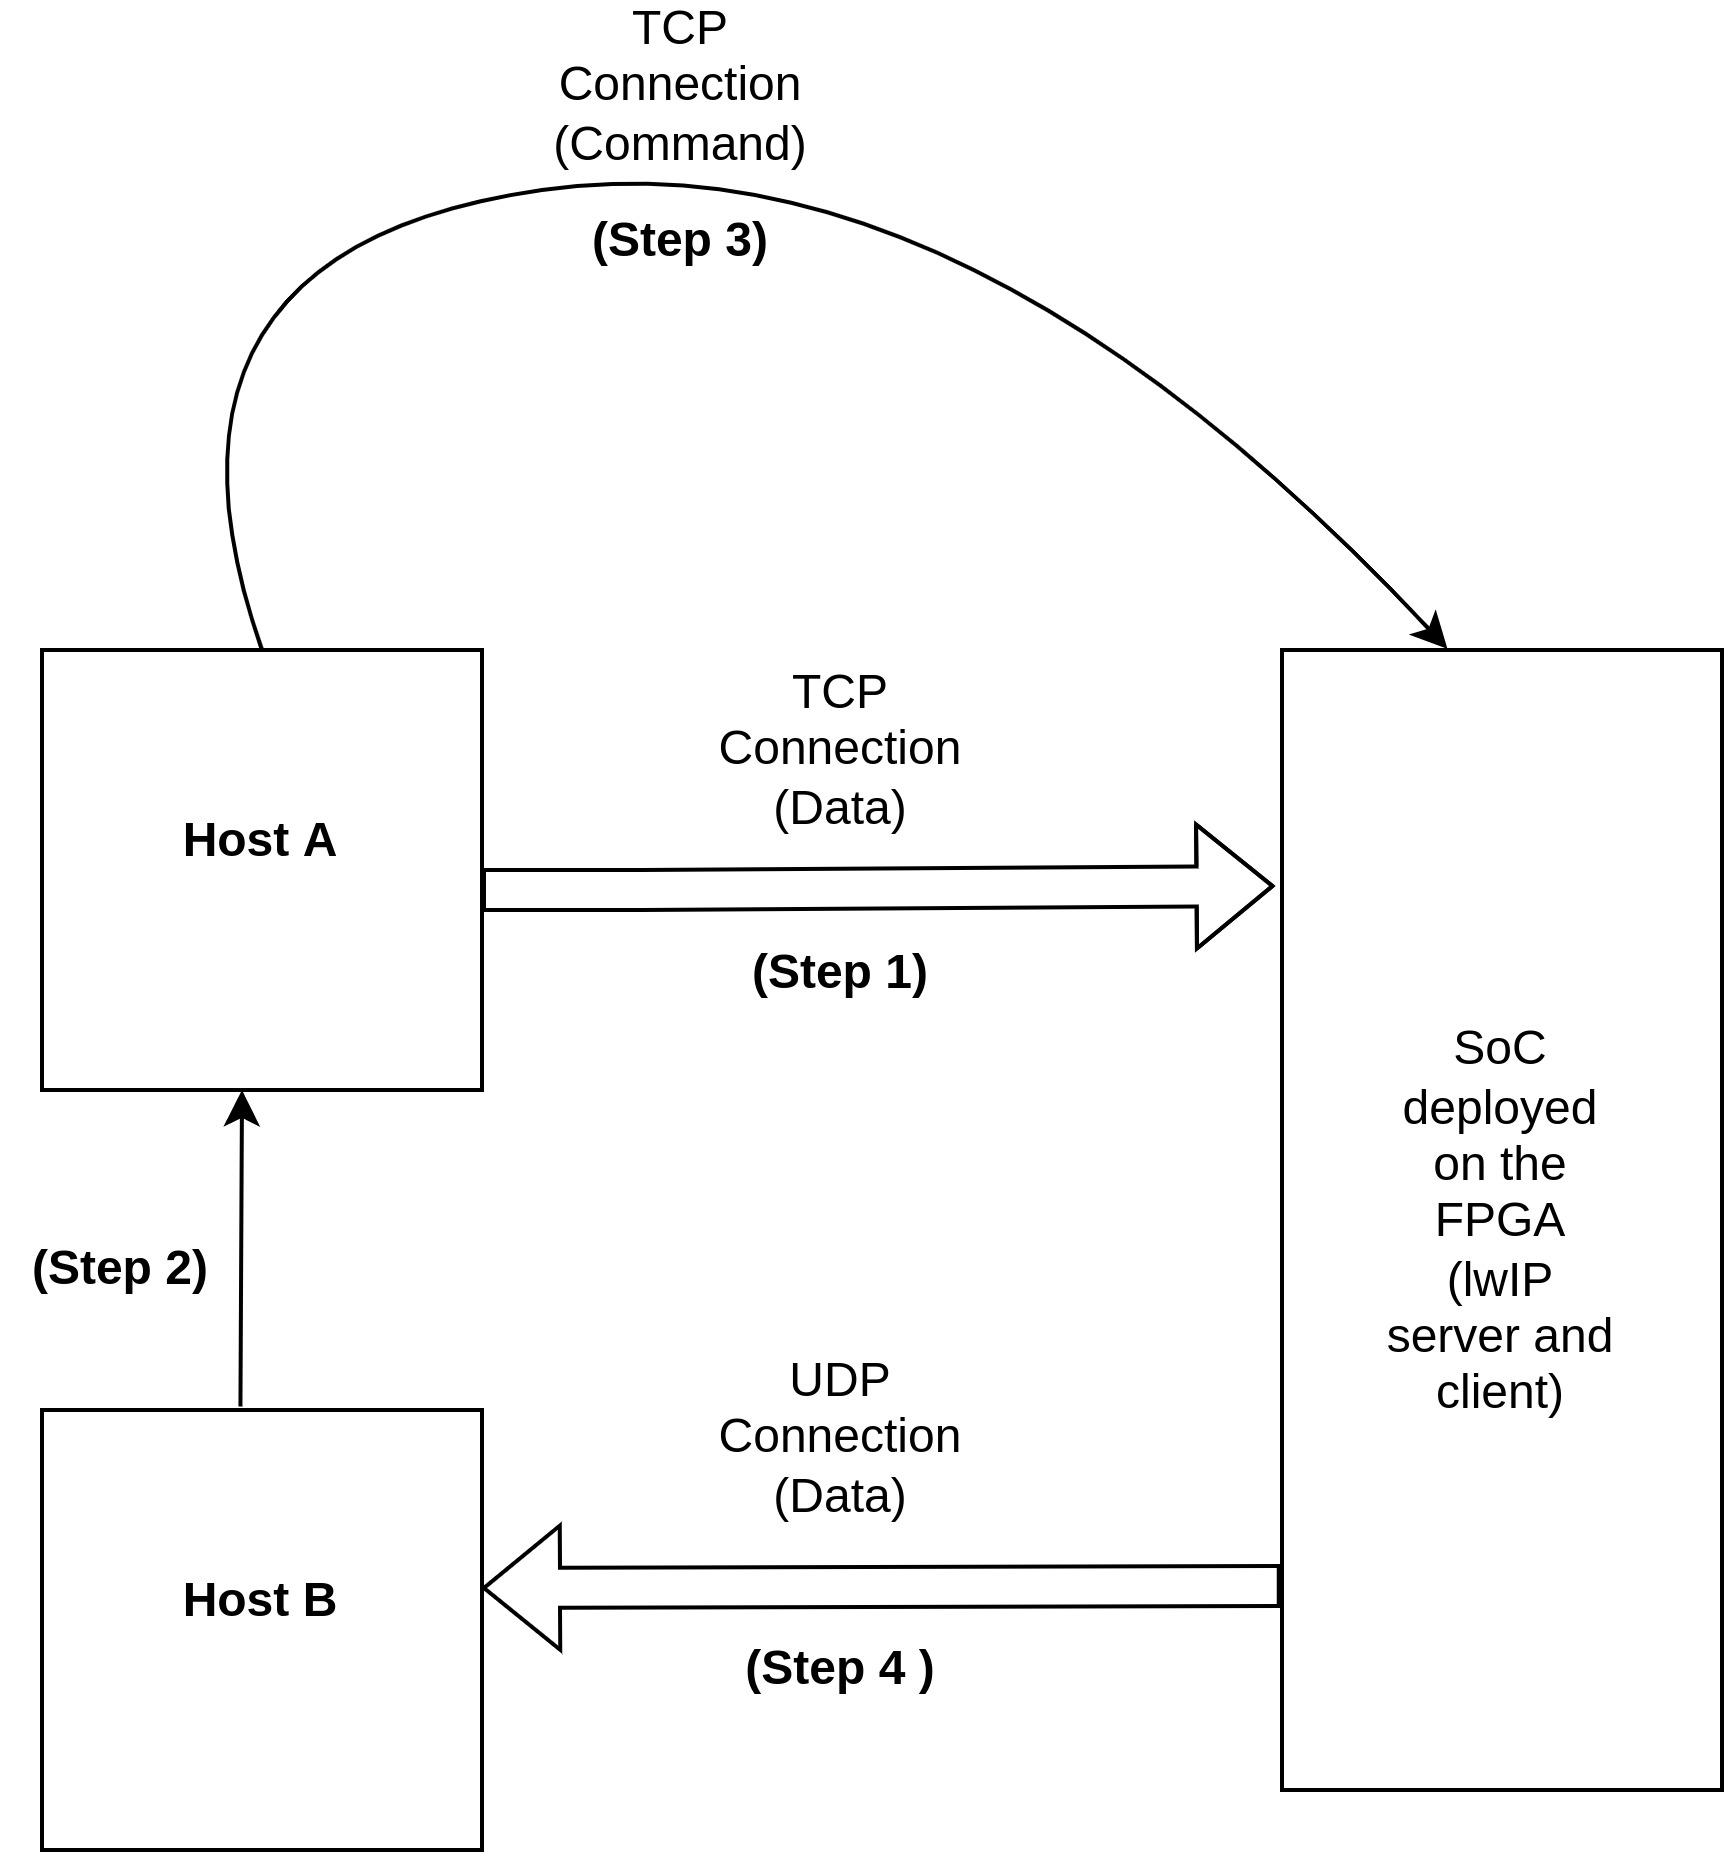
\includegraphics[width=12cm]{../figures/caching_app.jpg}
			\caption{Network caching application}
			\label{fig:NIC-Proc-top-level5}
		\end{figure}
  
\end{appendices}
\end{document}
%%%%%%%%%%%%%%%%%%%%%%%%%%%%%%%%%%%%%%%%%%%%%%%%%%%%%%%%%%%%%%%%%%%%%

